% Options for packages loaded elsewhere
\PassOptionsToPackage{unicode}{hyperref}
\PassOptionsToPackage{hyphens}{url}
%
\documentclass[
]{article}
\usepackage{amsmath,amssymb}
\usepackage{lmodern}
\usepackage{iftex}
\ifPDFTeX
  \usepackage[T1]{fontenc}
  \usepackage[utf8]{inputenc}
  \usepackage{textcomp} % provide euro and other symbols
\else % if luatex or xetex
  \usepackage{unicode-math}
  \defaultfontfeatures{Scale=MatchLowercase}
  \defaultfontfeatures[\rmfamily]{Ligatures=TeX,Scale=1}
\fi
% Use upquote if available, for straight quotes in verbatim environments
\IfFileExists{upquote.sty}{\usepackage{upquote}}{}
\IfFileExists{microtype.sty}{% use microtype if available
  \usepackage[]{microtype}
  \UseMicrotypeSet[protrusion]{basicmath} % disable protrusion for tt fonts
}{}
\makeatletter
\@ifundefined{KOMAClassName}{% if non-KOMA class
  \IfFileExists{parskip.sty}{%
    \usepackage{parskip}
  }{% else
    \setlength{\parindent}{0pt}
    \setlength{\parskip}{6pt plus 2pt minus 1pt}}
}{% if KOMA class
  \KOMAoptions{parskip=half}}
\makeatother
\usepackage{xcolor}
\IfFileExists{xurl.sty}{\usepackage{xurl}}{} % add URL line breaks if available
\IfFileExists{bookmark.sty}{\usepackage{bookmark}}{\usepackage{hyperref}}
\hypersetup{
  pdftitle={IRT-LSEM Phase 1 --- Final Report},
  pdfauthor={Pipeline output: B0 → B1 → B2 → B3 → B4 → B5},
  hidelinks,
  pdfcreator={LaTeX via pandoc}}
\urlstyle{same} % disable monospaced font for URLs
\usepackage[margin=1in]{geometry}
\usepackage{longtable,booktabs,array}
\usepackage{calc} % for calculating minipage widths
% Correct order of tables after \paragraph or \subparagraph
\usepackage{etoolbox}
\makeatletter
\patchcmd\longtable{\par}{\if@noskipsec\mbox{}\fi\par}{}{}
\makeatother
% Allow footnotes in longtable head/foot
\IfFileExists{footnotehyper.sty}{\usepackage{footnotehyper}}{\usepackage{footnote}}
\makesavenoteenv{longtable}
\usepackage{graphicx}
\makeatletter
\def\maxwidth{\ifdim\Gin@nat@width>\linewidth\linewidth\else\Gin@nat@width\fi}
\def\maxheight{\ifdim\Gin@nat@height>\textheight\textheight\else\Gin@nat@height\fi}
\makeatother
% Scale images if necessary, so that they will not overflow the page
% margins by default, and it is still possible to overwrite the defaults
% using explicit options in \includegraphics[width, height, ...]{}
\setkeys{Gin}{width=\maxwidth,height=\maxheight,keepaspectratio}
% Set default figure placement to htbp
\makeatletter
\def\fps@figure{htbp}
\makeatother
\setlength{\emergencystretch}{3em} % prevent overfull lines
\providecommand{\tightlist}{%
  \setlength{\itemsep}{0pt}\setlength{\parskip}{0pt}}
\setcounter{secnumdepth}{-\maxdimen} % remove section numbering
\ifLuaTeX
  \usepackage{selnolig}  % disable illegal ligatures
\fi

\title{IRT-LSEM Phase 1 --- Final Report}
\usepackage{etoolbox}
\makeatletter
\providecommand{\subtitle}[1]{% add subtitle to \maketitle
  \apptocmd{\@title}{\par {\large #1 \par}}{}{}
}
\makeatother
\subtitle{OLM Math THPT, School Year 2024-2025}
\author{Pipeline output: B0 → B1 → B2 → B3 → B4 → B5}
\date{2026-05-28}

\begin{document}
\maketitle

\hypertarget{introduction}{%
\section{1. Introduction}\label{introduction}}

\hypertarget{background-from-static-to-dynamic-ability}{%
\subsection{1.1 Background --- from static to dynamic
ability}\label{background-from-static-to-dynamic-ability}}

Classical Item Response Theory (IRT) treats a student's ability as a
single fixed quantity within a testing occasion. For the one-parameter
(Rasch) model, the probability that student \(i\) answers item \(j\)
correctly is

\[
P(Y_{ij} = 1 \mid \theta_i, b_j) = \sigma(\theta_i - b_j)
= \frac{\exp(\theta_i - b_j)}{1 + \exp(\theta_i - b_j)},
\]

where \(\theta_i\) is the latent ability and \(b_j\) the item
difficulty. This is adequate for a single exam, but on an online
learning system where a student engages repeatedly across a whole school
year, ability is not static: it should be indexed by time,
\(\theta_{it}\). Estimating the \emph{trajectory} \(\{\theta_{it}\}_t\)
--- and the structural process generating it --- is the goal of this
study.

We combine two layers. The \textbf{measurement layer} (IRT) converts
binary responses into a per-occasion ability estimate with measurement
error, producing \((\hat\theta_{it}, \mathrm{SE}_{it})\) via Bayesian
EAP scoring. The \textbf{structural layer} (LSEM/DSEM) models how
\(\theta_{it}\) evolves: a Latent Growth Curve Model (LGCM),

\[
\theta_{it} = \eta_{0i} + \eta_{1i}\,\lambda_t + \varepsilon_{it},
\]

a Latent Change Score Model (LCSM) whose coupling parameter \(\beta\)
captures whether weaker students catch up,

\[
\Delta\theta_{it} = \alpha + \beta\,\theta_{i,t-1} + \zeta_{it},
\]

and, for the intensively-measured Grade 12 subsample, a continuous-time
dynamic SEM (CT-DSEM) built on an Ornstein--Uhlenbeck process,

\[
d\theta_{it} = \left(\mu_i - \varphi_i\,\theta_{it}\right)dt + \sigma_i\,dW_t,
\]

with individual mean-reversion rate \(\varphi_i\) and equilibrium
\(\theta_{\text{eq}} = -c/\varphi\).

\hypertarget{research-gap}{%
\subsection{1.2 Research gap}\label{research-gap}}

Dynamic-ability modelling that integrates IRT with longitudinal SEM has,
to our knowledge, not been applied to a Vietnamese online learning
context. OLM provides an unusually large but \emph{irregularly spaced}
longitudinal record (the inter-occasion gap \(\Delta t\) spans five
orders of magnitude), which motivates continuous-time methods and a
careful per-grade calibration design (no cross-grade \(\theta\) linking
is possible in this single school year).

\hypertarget{research-questions}{%
\subsection{1.3 Research questions}\label{research-questions}}

\begin{itemize}
\tightlist
\item
  \textbf{RQ1.} Do math-ability trajectories show meaningful growth over
  a school year?
\item
  \textbf{RQ2.} Are the growth dynamics consistent across grades 10, 11,
  and 12?
\item
  \textbf{RQ3.} Do students at different ability levels follow distinct
  dynamic patterns --- \emph{catch-up} (\(\beta < 0\)) versus
  \emph{Matthew effect} (\(\beta > 0\))?
\end{itemize}

\hypertarget{executive-summary}{%
\section{2. Executive Summary}\label{executive-summary}}

This report presents the IRT-LSEM analysis of OLM Math THPT data for
school year 2024-2025, covering grades 10, 11, and 12 with
\textbf{per-grade IRT calibration} (no cross-grade linking) and
\textbf{longitudinal SEM} (LGCM + LCSM + lmer + CT-DSEM).

\textbf{Key findings:}

\begin{itemize}
\tightlist
\item
  \textbf{All LSEM models fit excellently} (CFI \textgreater{} .99,
  RMSEA \textless{} .04 across grades).
\item
  \textbf{Growth slopes are small and positive} for all 3 grades, with
  magnitude decreasing from grade 11 (0.028) \textgreater{} grade 10
  (0.015) \textgreater{} grade 12 (0.006) per occasion.
\item
  \textbf{Catch-up → plateau shift} is the headline finding: LCSM
  coupling \(\beta\) is clearly negative (catch-up) in Grade 10,
  marginal in Grade 11, and \(\approx 0\) (plateau) in Grade 12; CT-DSEM
  (grade 12) shows individual mean-reversion toward equilibrium
  \(\theta_{\text{eq}} \approx 0.65\) logit.
\item
  \textbf{Method comparison}: LGCM-lmer slope difference \textgreater{}
  0.005 attributed to method (FIML vs REML on differing data coverage),
  not nonlinear growth.
\end{itemize}

\hypertarget{data-pipeline}{%
\section{3. Data \& Pipeline}\label{data-pipeline}}

\begin{longtable}[]{@{}
  >{\raggedright\arraybackslash}p{(\columnwidth - 4\tabcolsep) * \real{0.2727}}
  >{\raggedright\arraybackslash}p{(\columnwidth - 4\tabcolsep) * \real{0.3636}}
  >{\raggedright\arraybackslash}p{(\columnwidth - 4\tabcolsep) * \real{0.3636}}@{}}
\toprule
\begin{minipage}[b]{\linewidth}\raggedright
Step
\end{minipage} & \begin{minipage}[b]{\linewidth}\raggedright
Method
\end{minipage} & \begin{minipage}[b]{\linewidth}\raggedright
Output
\end{minipage} \\
\midrule
\endhead
B0 --- Preprocess & Python (pandas) & response\_long per grade × \{exam,
practice\} \\
B1 --- Dimensionality & R (psych::omega bifactor) & ECV per grade;
documented as 1D approx. \\
B2 --- IRT calibration & R (mirt, 1PL/2PL) & item params per grade \\
B3 --- EAP scoring & R (mirt::fscores) & θ trajectory per (HS, day) \\
B4a --- LSEM Tier 1+2 & R (lavaan, lme4) & LGCM, LCSM, lmer params \\
B4c --- CT-DSEM & R (ctsem, optim) & continuous-time dynamics, grade
12 \\
B5 --- Report & R Markdown & this document \\
\bottomrule
\end{longtable}

\hypertarget{sample-sizes}{%
\subsection{3.1 Sample sizes}\label{sample-sizes}}

\begin{longtable}[]{@{}rrrrr@{}}
\caption{Sample sizes per grade (after B3 EAP scoring)}\tabularnewline
\toprule
Grade & N\_HS & N\_obs & T\_median & T\_max \\
\midrule
\endfirsthead
\toprule
Grade & N\_HS & N\_obs & T\_median & T\_max \\
\midrule
\endhead
10 & 6407 & 32191 & 4 & 18 \\
11 & 7002 & 29959 & 4 & 17 \\
12 & 10804 & 60807 & 4 & 37 \\
\bottomrule
\end{longtable}

\hypertarget{irt-calibration-b2}{%
\subsection{3.2 IRT calibration (B2)}\label{irt-calibration-b2}}

\begin{itemize}
\tightlist
\item
  \textbf{Model}: 1PL (Rasch) per grade --- chosen over 2PL due to 2-6\%
  degenerate items in 2PL fits.
\item
  \textbf{Estimator}: mirt SQUAREM, 1500 iterations, 41 quadrature
  points (grade 12 only).
\item
  \textbf{Items}: G10=3,277; G11=3,473; G12=8,236 unique items.
\item
  \textbf{Itemfit}: S-X2 unavailable due to sparse data (each HS sees
  \textless{} 10\% of item pool); X2/infit used as alternative.
\end{itemize}

Diagnostic plots below use \textbf{Grade 12} as representative; grade
10/11 versions are in \texttt{outputs/b2\_calibration/plots/}.

\begin{figure}
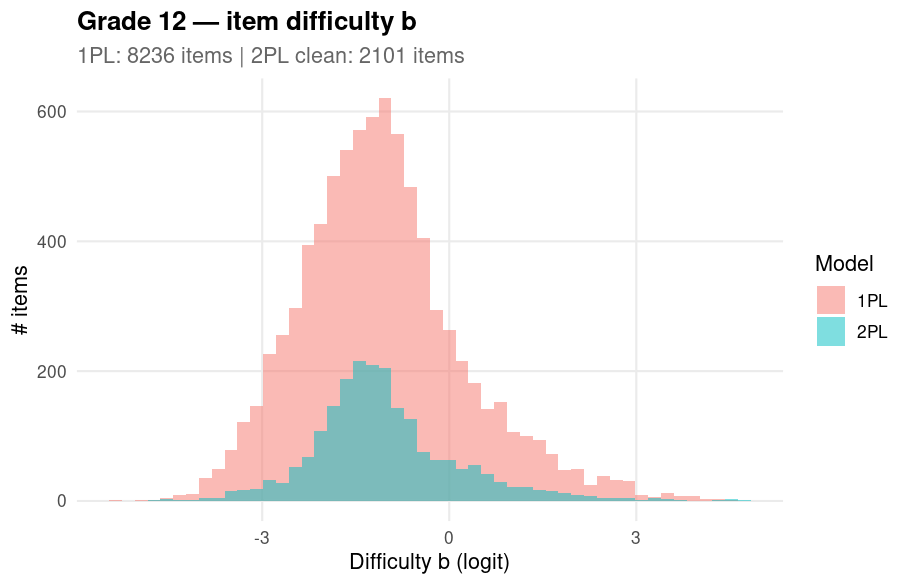
\includegraphics[width=0.49\linewidth]{../../outputs/b2_calibration/plots/difficulty_dist_grade_12} 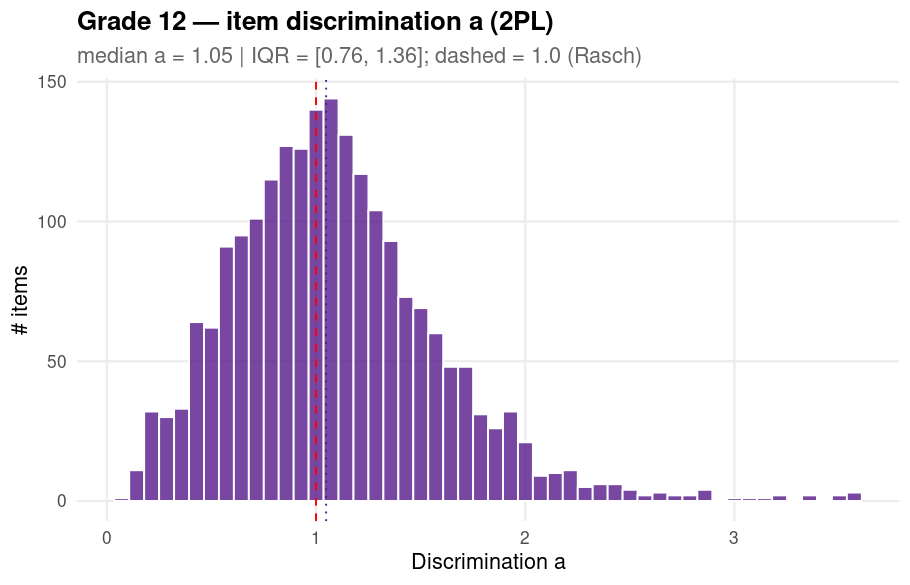
\includegraphics[width=0.49\linewidth]{../../outputs/b2_calibration/plots/discrimination_dist_grade_12} 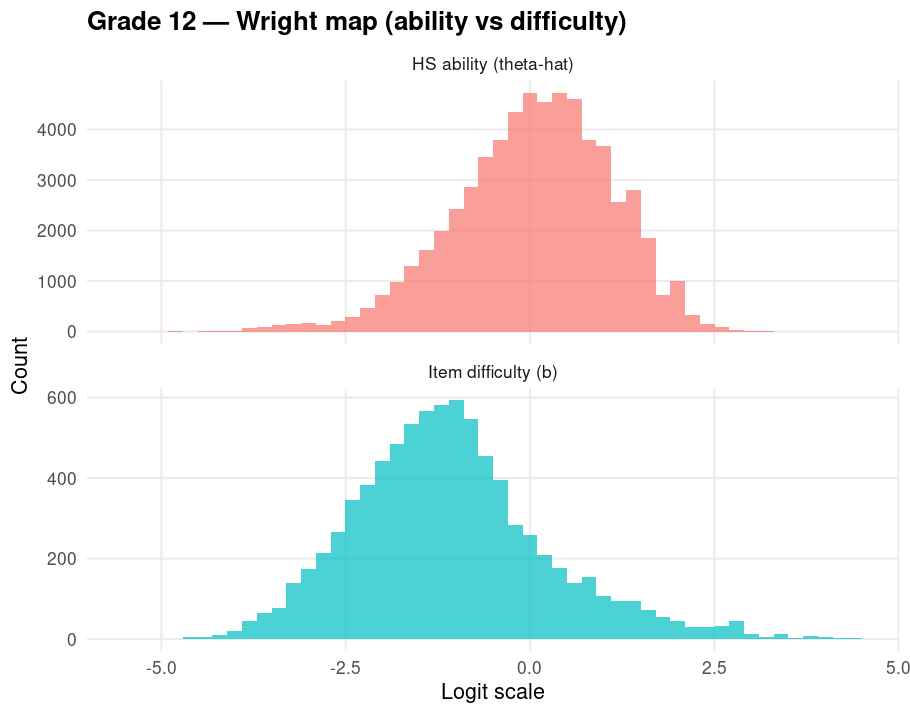
\includegraphics[width=0.49\linewidth]{../../outputs/b2_calibration/plots/wright_map_grade_12} 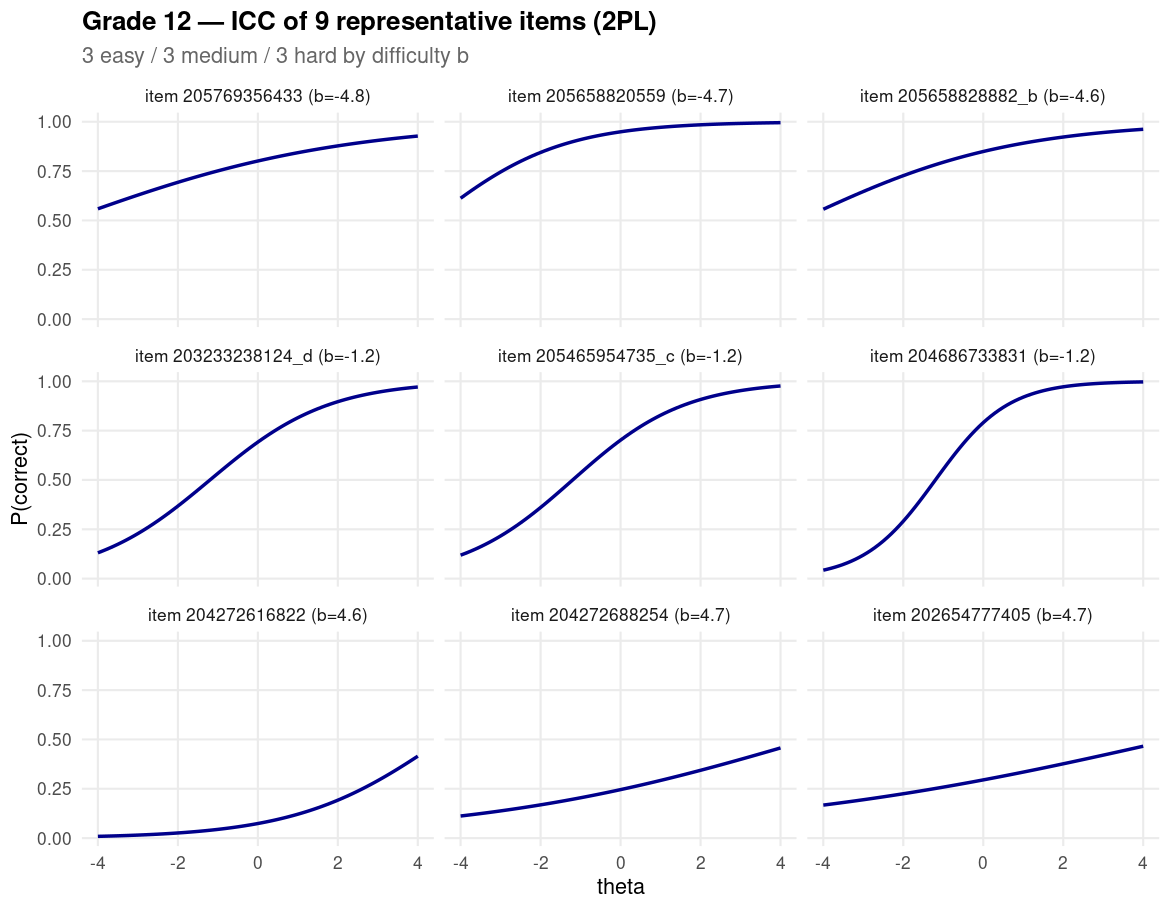
\includegraphics[width=0.49\linewidth]{../../outputs/b2_calibration/plots/icc_grade_12} \caption{ICC of 9 representative items (2PL).}\label{fig:b2-plots}
\end{figure}

The discrimination distribution (median \(a \approx\) values \(> 1\),
wide spread) is the empirical justification for considering 2PL; the
Wright map shows the item difficulties broadly cover the ability range,
with thin coverage at the extremes.

\hypertarget{data-shape-dimensionality}{%
\subsection{3.3 Data shape \&
dimensionality}\label{data-shape-dimensionality}}

Per-occasion counts (\(T_i\)) are right-skewed (median 4-5 days), and
inter-occasion gaps \(\Delta t\) span several orders of magnitude ---
motivating the continuous-time treatment in §7. The B1 scree plots
support a dominant first dimension (1D approximation adopted, with the
sparse-matrix caveat noted in §10).

\begin{figure}
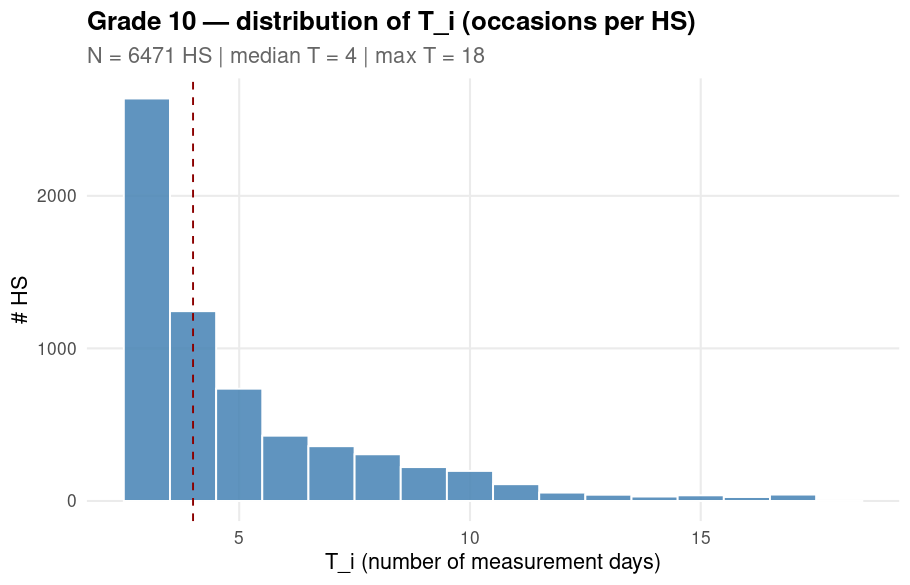
\includegraphics[width=0.32\linewidth]{../../outputs/b0_preprocessed/plots/T_distribution_grade_10} 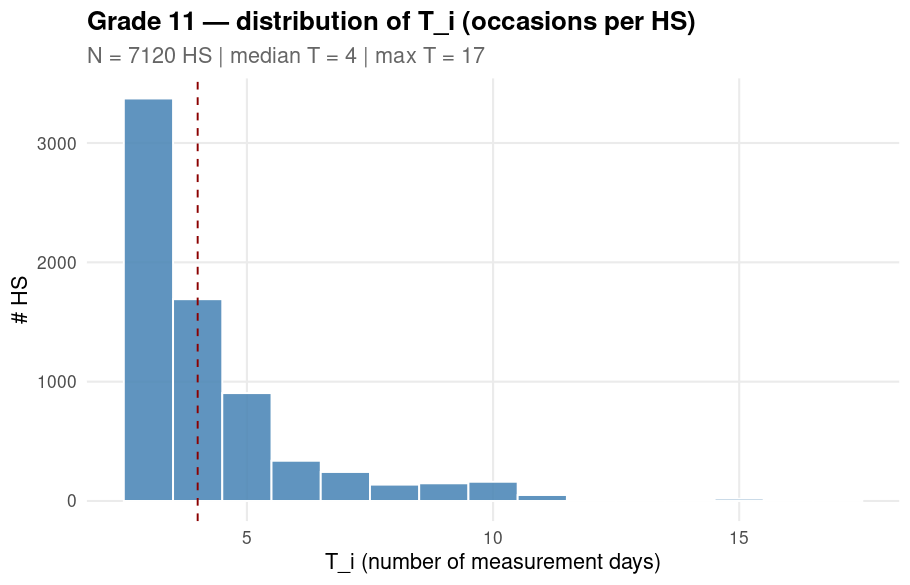
\includegraphics[width=0.32\linewidth]{../../outputs/b0_preprocessed/plots/T_distribution_grade_11} 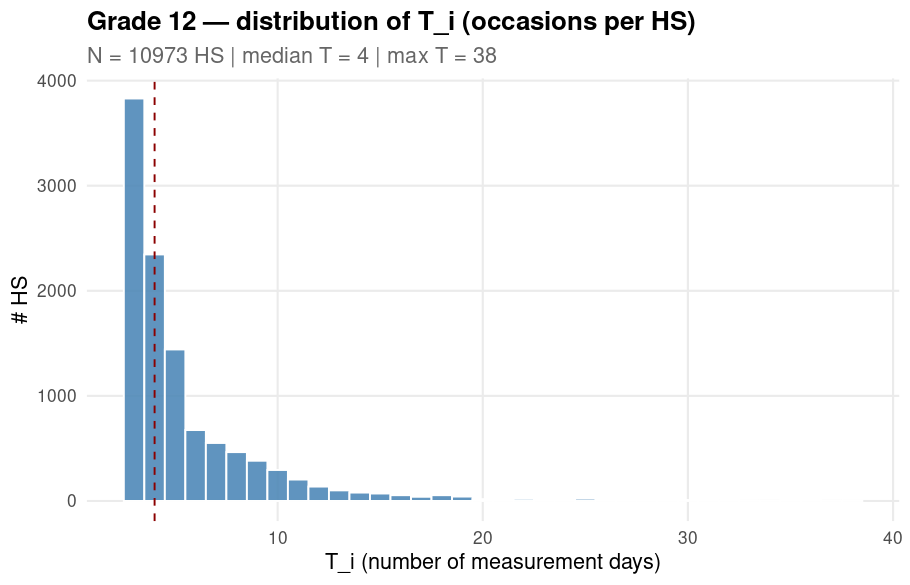
\includegraphics[width=0.32\linewidth]{../../outputs/b0_preprocessed/plots/T_distribution_grade_12} \caption{Grade 12 T\_i}\label{fig:b0-T-plots}
\end{figure}

\begin{figure}
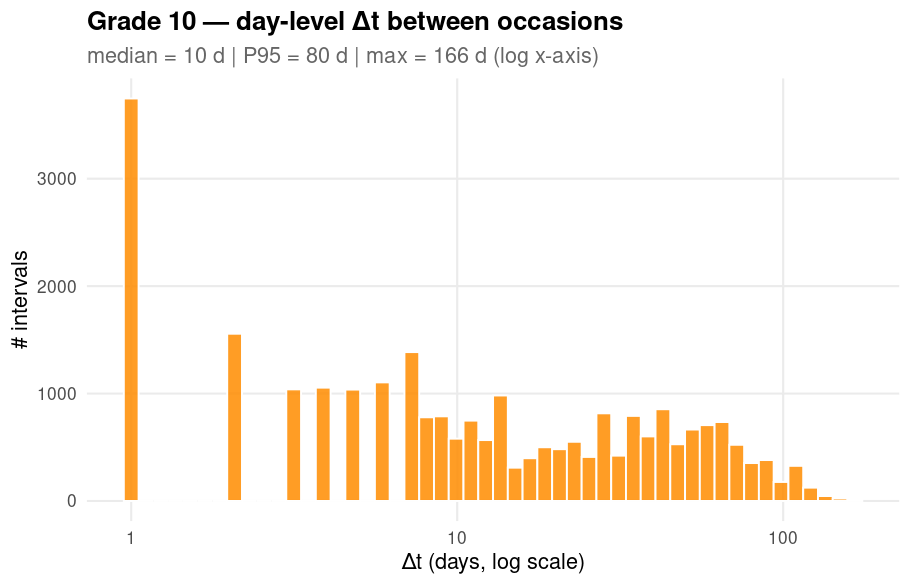
\includegraphics[width=0.32\linewidth]{../../outputs/b0_preprocessed/plots/dt_distribution_grade_10} 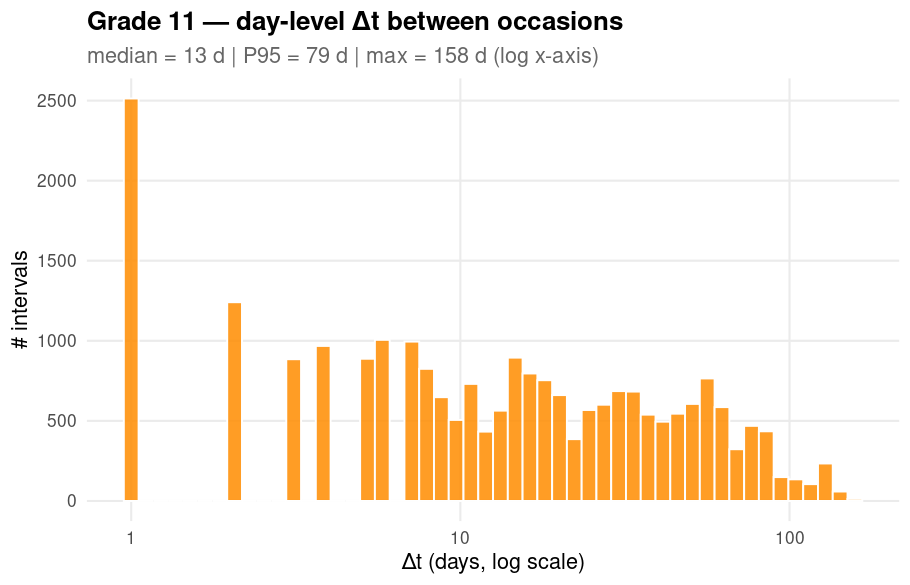
\includegraphics[width=0.32\linewidth]{../../outputs/b0_preprocessed/plots/dt_distribution_grade_11} 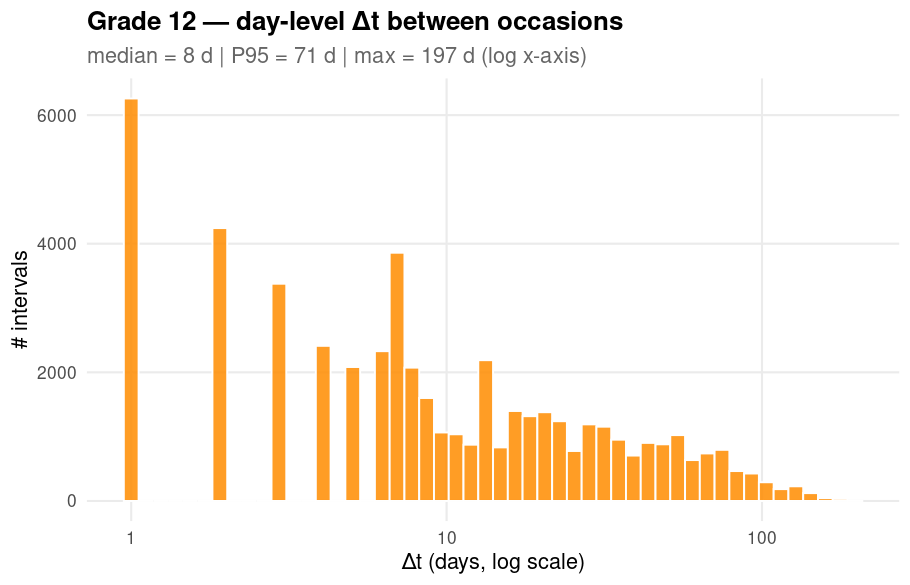
\includegraphics[width=0.32\linewidth]{../../outputs/b0_preprocessed/plots/dt_distribution_grade_12} \caption{Grade 12 Δt}\label{fig:b0-dt-plots}
\end{figure}

\begin{figure}
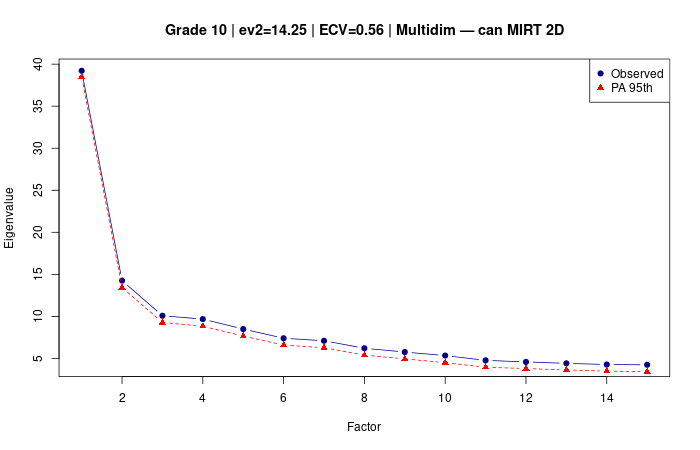
\includegraphics[width=0.32\linewidth]{../../outputs/b1_dimensionality/scree_plot_grade_10} 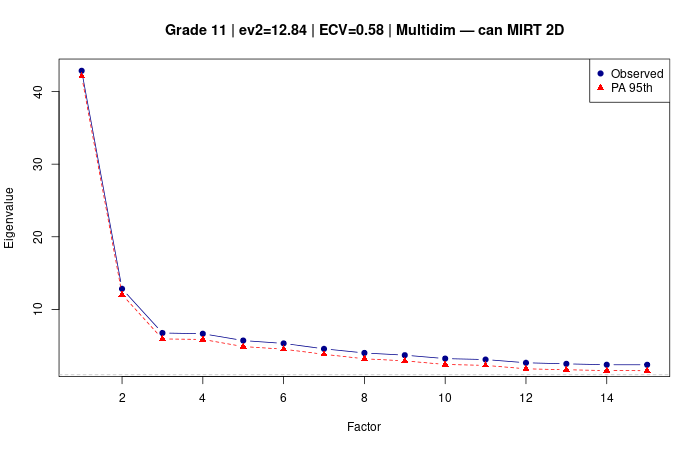
\includegraphics[width=0.32\linewidth]{../../outputs/b1_dimensionality/scree_plot_grade_11} 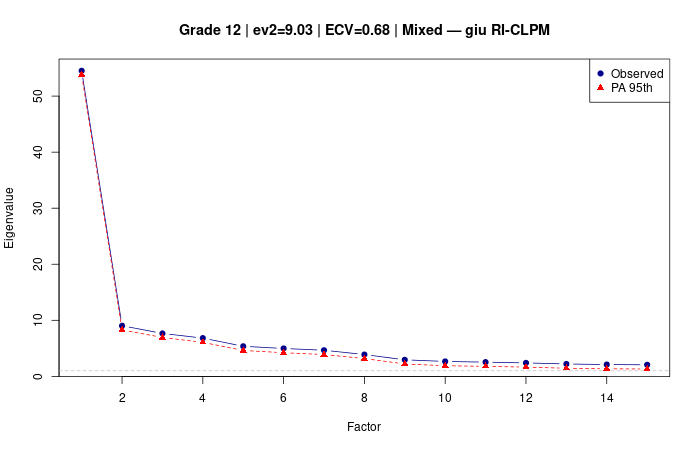
\includegraphics[width=0.32\linewidth]{../../outputs/b1_dimensionality/scree_plot_grade_12} \caption{Grade 12 scree}\label{fig:b1-scree}
\end{figure}

\hypertarget{measurement-quality-b3-eap}{%
\subsection{3.4 Measurement quality (B3
EAP)}\label{measurement-quality-b3-eap}}

\begin{longtable}[]{@{}rrrrr@{}}
\caption{Empirical reliability rho = 1 -
mean(SE\^{}2)/Var(theta-hat)}\tabularnewline
\toprule
Grade & N\_obs & Var\_theta & Mean\_SE2 & Reliability \\
\midrule
\endfirsthead
\toprule
Grade & N\_obs & Var\_theta & Mean\_SE2 & Reliability \\
\midrule
\endhead
10 & 32191 & 0.835 & 0.261 & 0.687 \\
11 & 29959 & 1.161 & 0.295 & 0.746 \\
12 & 60807 & 1.107 & 0.206 & 0.814 \\
\bottomrule
\end{longtable}

Reliability is acceptable for research (Grade 12 = 0.81, Grade 11 =
0.75); Grade 10 (0.69) sits just below the conventional 0.70 threshold,
consistent with its shorter, less informative tests. Diagnostic
distributions (Grade 12 representative; grades 10/11 in
\texttt{outputs/b3\_theta/plots/}):

\begin{figure}
\includegraphics[width=0.49\linewidth]{../../outputs/b3_theta/plots/trajectory_samples_grade_12} 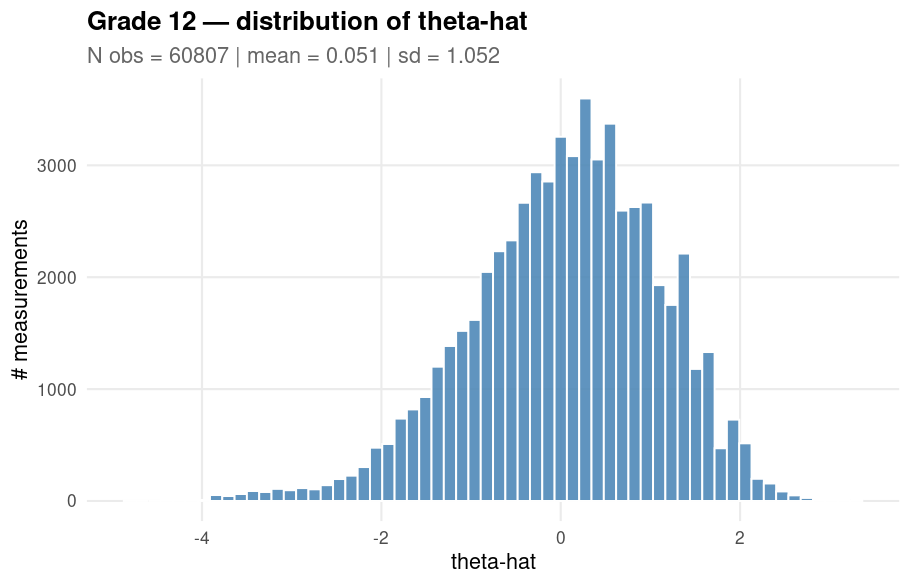
\includegraphics[width=0.49\linewidth]{../../outputs/b3_theta/plots/theta_distribution_grade_12} 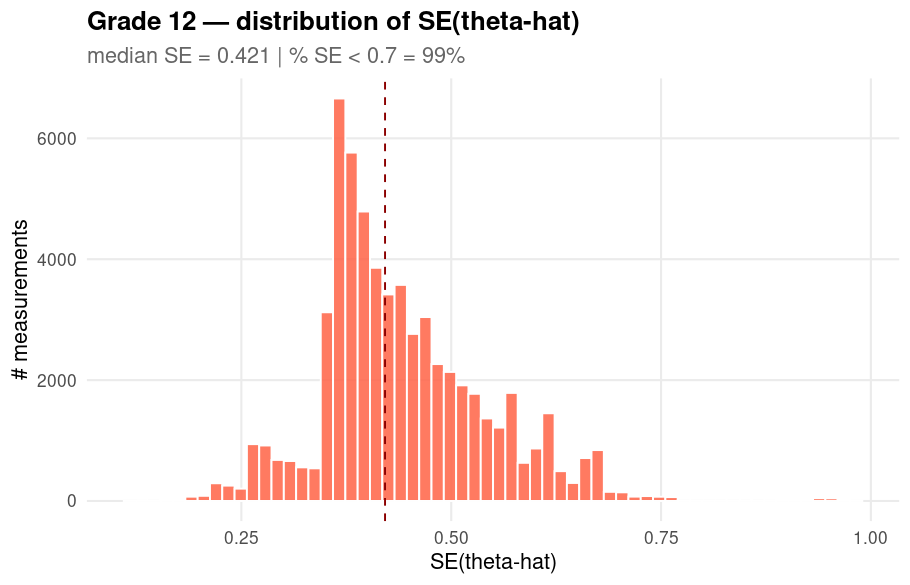
\includegraphics[width=0.49\linewidth]{../../outputs/b3_theta/plots/se_distribution_grade_12} \caption{SE(theta-hat) distribution.}\label{fig:b3-plots}
\end{figure}

\hypertarget{main-results-figure}{%
\section{4. Main Results Figure}\label{main-results-figure}}

The four panels below summarise the study's headline results:
cross-grade growth trajectories (a), the \textbf{catch-up → plateau}
coupling shift (b), slope agreement across estimation methods (c), and
the continuous-time learning-rate regime in Grade 12 (d).

\begin{figure}
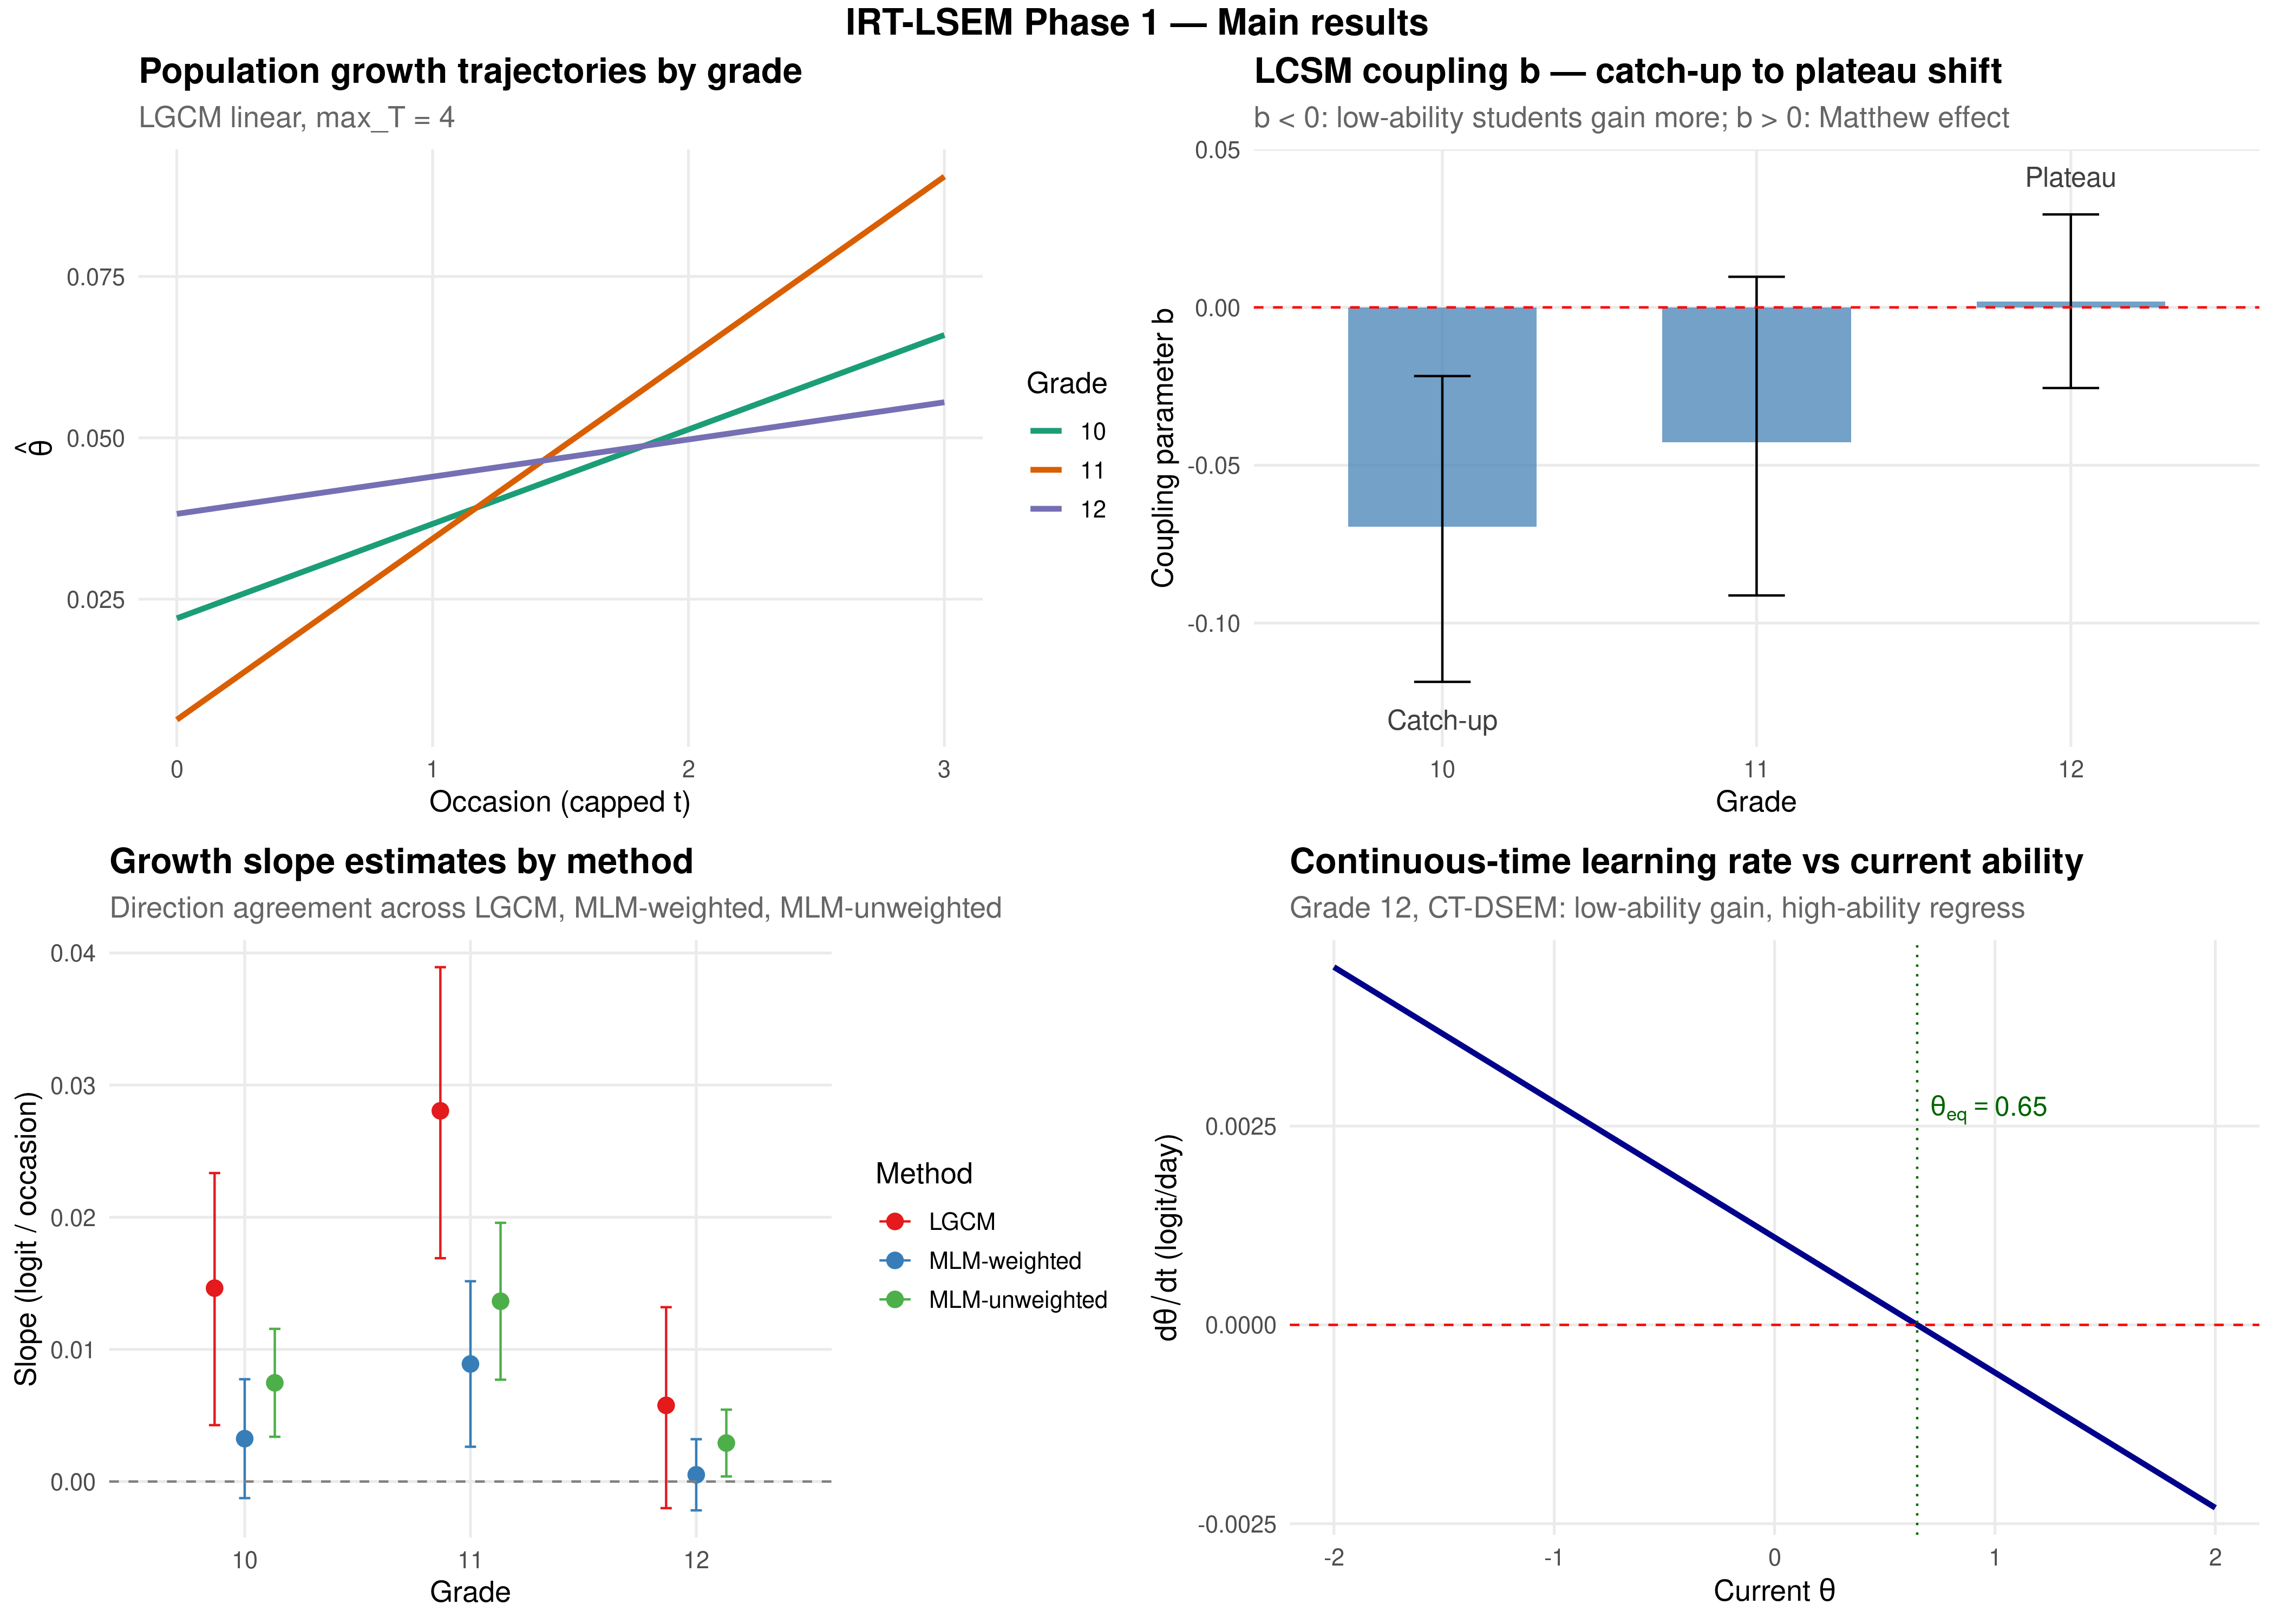
\includegraphics[width=1\linewidth]{../../outputs/b5_report/fig_main_results} \caption{Main results. (a) LGCM population trajectories by grade. (b) LCSM coupling b — the catch-up to plateau shift (KEY FINDING). (c) Growth slope by method (LGCM / MLM-weighted / MLM-unweighted). (d) CT-DSEM learning rate vs current ability, Grade 12.}\label{fig:main-figure}
\end{figure}

\hypertarget{longitudinal-sem-tier-1-b4a-lgcm-lcsm}{%
\section{5. Longitudinal SEM Tier 1 (B4a) --- LGCM +
LCSM}\label{longitudinal-sem-tier-1-b4a-lgcm-lcsm}}

\hypertarget{fit-indices}{%
\subsection{5.1 Fit indices}\label{fit-indices}}

\begin{longtable}[]{@{}
  >{\raggedright\arraybackslash}p{(\columnwidth - 20\tabcolsep) * \real{0.0789}}
  >{\raggedleft\arraybackslash}p{(\columnwidth - 20\tabcolsep) * \real{0.0789}}
  >{\raggedleft\arraybackslash}p{(\columnwidth - 20\tabcolsep) * \real{0.0789}}
  >{\raggedleft\arraybackslash}p{(\columnwidth - 20\tabcolsep) * \real{0.0395}}
  >{\raggedleft\arraybackslash}p{(\columnwidth - 20\tabcolsep) * \real{0.1184}}
  >{\raggedleft\arraybackslash}p{(\columnwidth - 20\tabcolsep) * \real{0.0789}}
  >{\raggedleft\arraybackslash}p{(\columnwidth - 20\tabcolsep) * \real{0.0789}}
  >{\raggedleft\arraybackslash}p{(\columnwidth - 20\tabcolsep) * \real{0.0789}}
  >{\raggedright\arraybackslash}p{(\columnwidth - 20\tabcolsep) * \real{0.1974}}
  >{\raggedleft\arraybackslash}p{(\columnwidth - 20\tabcolsep) * \real{0.0789}}
  >{\raggedleft\arraybackslash}p{(\columnwidth - 20\tabcolsep) * \real{0.0921}}@{}}
\caption{Fit indices for LGCM and LCSM models, grades 10-12
(max\_T=4)}\tabularnewline
\toprule
\begin{minipage}[b]{\linewidth}\raggedright
Model
\end{minipage} & \begin{minipage}[b]{\linewidth}\raggedleft
Grade
\end{minipage} & \begin{minipage}[b]{\linewidth}\raggedleft
ChiSq
\end{minipage} & \begin{minipage}[b]{\linewidth}\raggedleft
df
\end{minipage} & \begin{minipage}[b]{\linewidth}\raggedleft
p
\end{minipage} & \begin{minipage}[b]{\linewidth}\raggedleft
CFI
\end{minipage} & \begin{minipage}[b]{\linewidth}\raggedleft
TLI
\end{minipage} & \begin{minipage}[b]{\linewidth}\raggedleft
RMSEA
\end{minipage} & \begin{minipage}[b]{\linewidth}\raggedright
RMSEA\_CI
\end{minipage} & \begin{minipage}[b]{\linewidth}\raggedleft
SRMR
\end{minipage} & \begin{minipage}[b]{\linewidth}\raggedleft
BIC
\end{minipage} \\
\midrule
\endfirsthead
\toprule
\begin{minipage}[b]{\linewidth}\raggedright
Model
\end{minipage} & \begin{minipage}[b]{\linewidth}\raggedleft
Grade
\end{minipage} & \begin{minipage}[b]{\linewidth}\raggedleft
ChiSq
\end{minipage} & \begin{minipage}[b]{\linewidth}\raggedleft
df
\end{minipage} & \begin{minipage}[b]{\linewidth}\raggedleft
p
\end{minipage} & \begin{minipage}[b]{\linewidth}\raggedleft
CFI
\end{minipage} & \begin{minipage}[b]{\linewidth}\raggedleft
TLI
\end{minipage} & \begin{minipage}[b]{\linewidth}\raggedleft
RMSEA
\end{minipage} & \begin{minipage}[b]{\linewidth}\raggedright
RMSEA\_CI
\end{minipage} & \begin{minipage}[b]{\linewidth}\raggedleft
SRMR
\end{minipage} & \begin{minipage}[b]{\linewidth}\raggedleft
BIC
\end{minipage} \\
\midrule
\endhead
LGCM & 10 & 17.08 & 5 & 4.36e-03 & 0.996 & 0.996 & 0.019 & {[}0.010,
0.030{]} & 0.011 & 57703 \\
LCSM & 10 & 7.11 & 2 & 2.85e-02 & 0.998 & 0.995 & 0.020 & {[}0.006,
0.037{]} & 0.008 & 57720 \\
LGCM & 11 & 38.45 & 5 & 3.00e-07 & 0.991 & 0.989 & 0.031 & {[}0.022,
0.040{]} & 0.017 & 69015 \\
LCSM & 11 & 6.81 & 2 & 3.32e-02 & 0.999 & 0.996 & 0.019 & {[}0.004,
0.035{]} & 0.007 & 69010 \\
LGCM & 12 & 32.50 & 5 & 4.70e-06 & 0.997 & 0.996 & 0.023 & {[}0.016,
0.030{]} & 0.011 & 105984 \\
LCSM & 12 & 15.20 & 2 & 5.01e-04 & 0.998 & 0.995 & 0.025 & {[}0.014,
0.037{]} & 0.010 & 105995 \\
\bottomrule
\end{longtable}

All models meet conventional cutoffs (CFI \textgreater{} .95, RMSEA
\textless{} .06, SRMR \textless{} .08). LCSM provides marginal BIC
improvement over LGCM for grade 11 only.

\hypertarget{lgcm-growth-parameters}{%
\subsection{5.2 LGCM growth parameters}\label{lgcm-growth-parameters}}

\begin{longtable}[]{@{}rlrl@{}}
\caption{LGCM parameters with 1000-bootstrap 95\% CI}\tabularnewline
\toprule
Grade & Param & Estimate & CI \\
\midrule
\endfirsthead
\toprule
Grade & Param & Estimate & CI \\
\midrule
\endhead
10 & i\_mean & 0.0220 & {[}0.0006, 0.0440{]} \\
10 & s\_mean & 0.0146 & {[}0.0043, 0.0233{]} \\
10 & i\_var & 0.3295 & --- \\
10 & s\_var & 0.0218 & --- \\
11 & i\_mean & 0.0063 & {[}-0.0154, 0.0285{]} \\
11 & s\_mean & 0.0281 & {[}0.0169, 0.0389{]} \\
11 & i\_var & 0.4253 & --- \\
11 & s\_var & 0.0352 & --- \\
12 & i\_mean & 0.0382 & {[}0.0206, 0.0573{]} \\
12 & s\_mean & 0.0058 & {[}-0.0020, 0.0132{]} \\
12 & i\_var & 0.4659 & --- \\
12 & s\_var & 0.0157 & --- \\
\bottomrule
\end{longtable}

\textbf{Interpretation:}

\begin{itemize}
\tightlist
\item
  \texttt{i\_mean}: starting \(\theta\) (intercept factor mean) ---
  small, positive across grades.
\item
  \texttt{s\_mean}: linear growth rate per occasion (out of 4) --- Grade
  11 highest (0.028), Grade 12 lowest (0.006).
\item
  Variances \texttt{i\_var}, \texttt{s\_var} represent between-HS
  heterogeneity in starting level and growth rate.
\end{itemize}

\begin{figure}
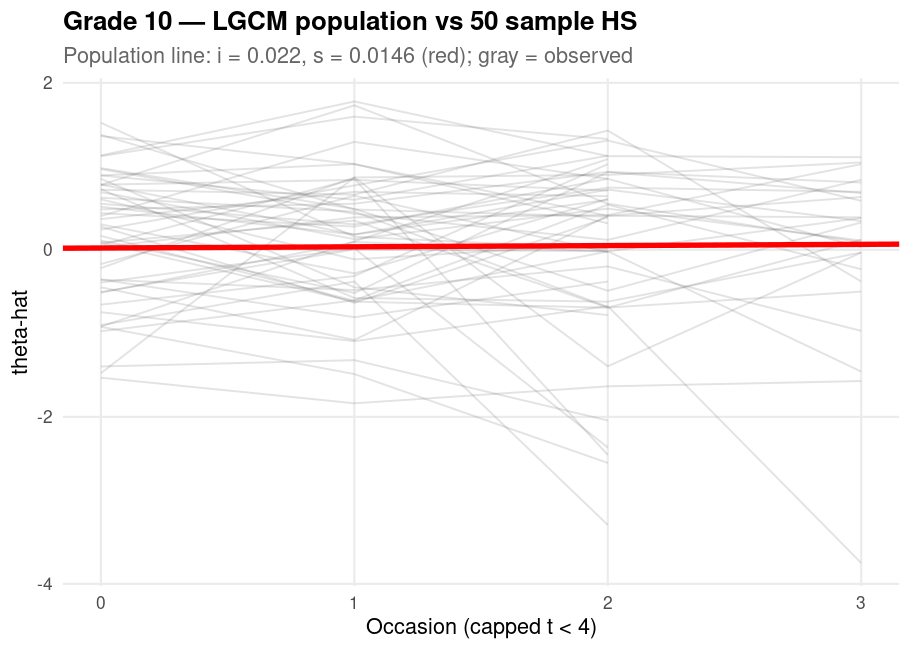
\includegraphics[width=0.32\linewidth]{../../outputs/b4_lsem/plots/lgcm_overlay_grade_10} 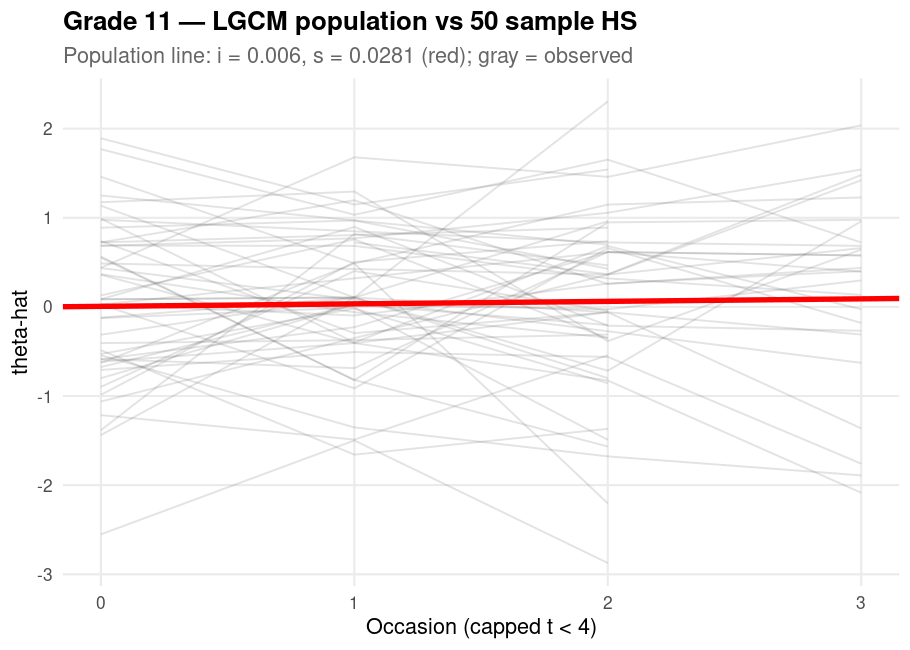
\includegraphics[width=0.32\linewidth]{../../outputs/b4_lsem/plots/lgcm_overlay_grade_11} 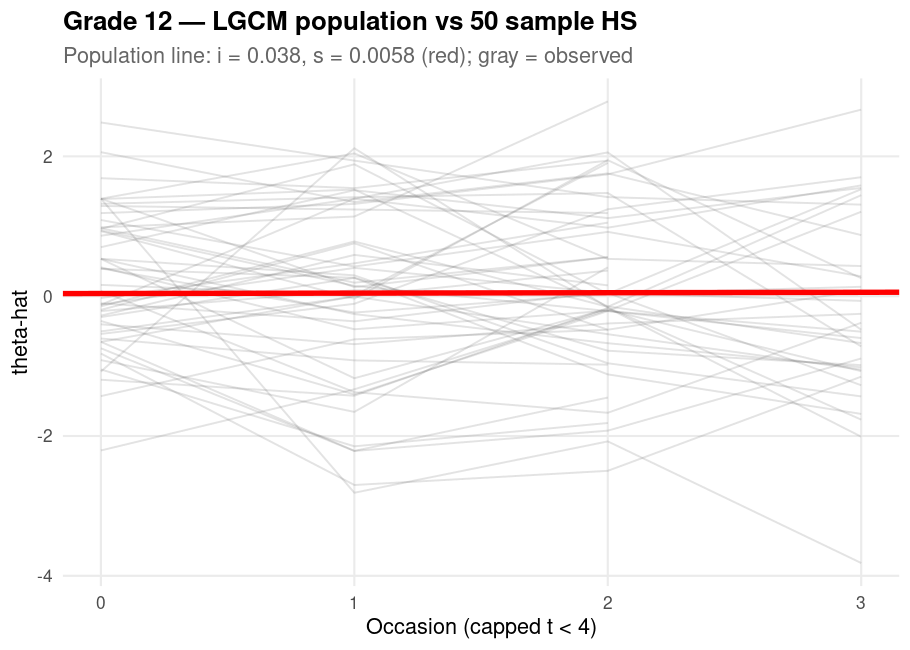
\includegraphics[width=0.32\linewidth]{../../outputs/b4_lsem/plots/lgcm_overlay_grade_12} \caption{Grade 12}\label{fig:lgcm-overlay}
\end{figure}

The red population line (intercept + slope) overlays 50 sampled observed
trajectories, showing the small positive average growth against
substantial between-student spread.

\hypertarget{lcsm-coupling-catch-up-vs-matthew-effect-key-finding}{%
\subsection{5.3 LCSM coupling --- catch-up vs Matthew effect (KEY
FINDING)}\label{lcsm-coupling-catch-up-vs-matthew-effect-key-finding}}

\begin{longtable}[]{@{}rlrl@{}}
\caption{LCSM parameters with 1000-bootstrap 95\% CI}\tabularnewline
\toprule
Grade & Param & Estimate & CI \\
\midrule
\endfirsthead
\toprule
Grade & Param & Estimate & CI \\
\midrule
\endhead
10 & b & -0.0695 & {[}-0.1186, -0.0218{]} \\
10 & alpha & 0.0087 & {[}0.0035, 0.0143{]} \\
10 & alpha0 & 0.0070 & {[}-0.0141, 0.0296{]} \\
11 & b & -0.0427 & {[}-0.0912, 0.0097{]} \\
11 & alpha & 0.0199 & {[}0.0138, 0.0264{]} \\
11 & alpha0 & 0.0049 & {[}-0.0178, 0.0296{]} \\
12 & b & 0.0018 & {[}-0.0255, 0.0295{]} \\
12 & alpha & 0.0027 & {[}-0.0016, 0.0070{]} \\
12 & alpha0 & 0.0212 & {[}0.0012, 0.0399{]} \\
\bottomrule
\end{longtable}

\textbf{Coupling parameter \(\beta\) (reported as \texttt{b})
interpretation:}

\begin{itemize}
\tightlist
\item
  \(\beta < 0\) → \textbf{catch-up}: lower-\(\theta\) students gain more
  between occasions.
\item
  \(\beta > 0\) → \textbf{Matthew effect}: high-\(\theta\) students gain
  more.
\item
  \(\beta \approx 0\) → no coupling (plateau).
\end{itemize}

Result: Grade 10 shows clear catch-up (\(\beta = -0.069\), CI excludes
0); Grade 11 marginal catch-up (\(\beta = -0.043\), CI crosses 0); Grade
12 no coupling (\(\beta \approx 0\)). This grade-ordered weakening of
catch-up is the \textbf{catch-up → plateau shift} highlighted throughout
this report.

The change-score densities below split each grade by initial-ability
tercile. In Grade 10 the low-\(\theta_0\) group's \(\Delta\theta\) mass
sits visibly to the right of the high-\(\theta_0\) group (compensatory
catch-up); by Grade 12 the terciles overlap (plateau).

\begin{figure}
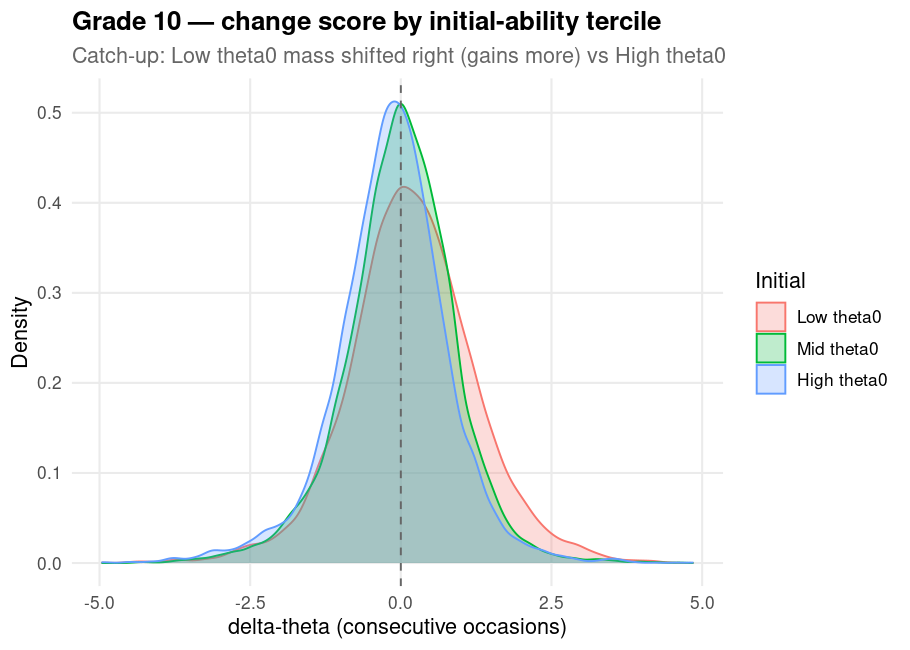
\includegraphics[width=0.32\linewidth]{../../outputs/b4_lsem/plots/lcsm_dtheta_density_grade_10} 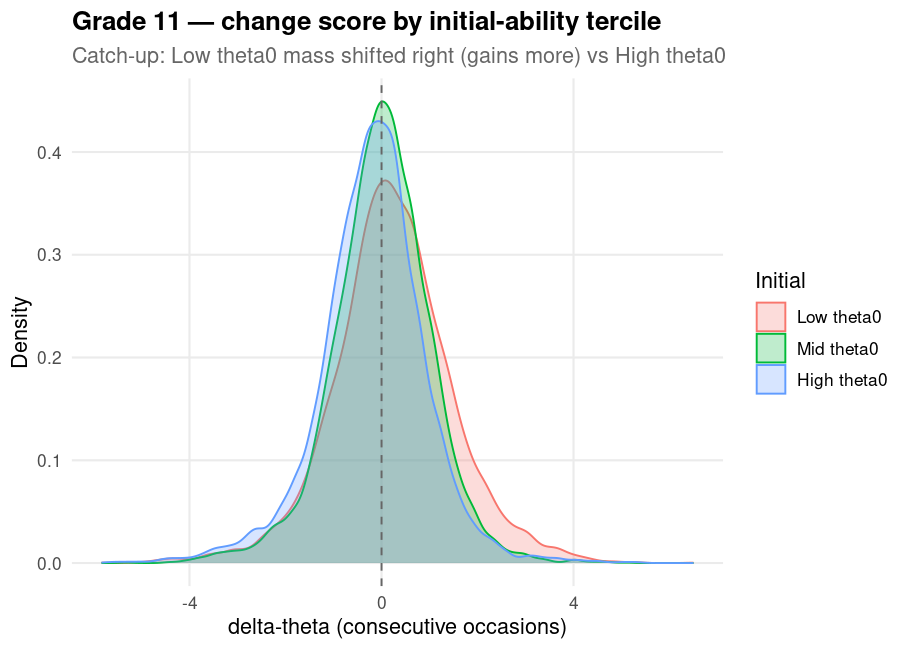
\includegraphics[width=0.32\linewidth]{../../outputs/b4_lsem/plots/lcsm_dtheta_density_grade_11} 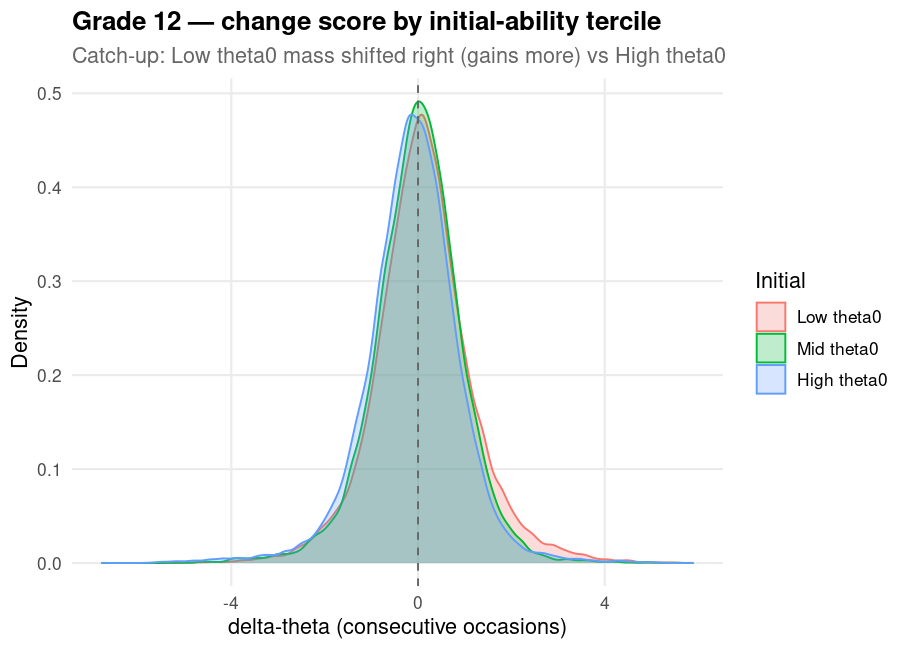
\includegraphics[width=0.32\linewidth]{../../outputs/b4_lsem/plots/lcsm_dtheta_density_grade_12} \caption{Grade 12}\label{fig:lcsm-density}
\end{figure}

\hypertarget{tier-2-mixed-effects-model-lmer}{%
\section{6. Tier 2 --- Mixed-effects Model
(lmer)}\label{tier-2-mixed-effects-model-lmer}}

\hypertarget{lmer-parameters-full-data-all-t-precision-weighted}{%
\subsection{6.1 lmer parameters (full data, all T,
precision-weighted)}\label{lmer-parameters-full-data-all-t-precision-weighted}}

\begin{longtable}[]{@{}rlrr@{}}
\caption{Mixed-effects model: theta \textasciitilde{} day\_idx +
(1+day\_idx\textbar iduser), weights=1/se\^{}2}\tabularnewline
\toprule
grade & param & est & se \\
\midrule
\endfirsthead
\toprule
grade & param & est & se \\
\midrule
\endhead
10 & intercept\_fixed & -0.0613 & 0.0096 \\
10 & slope\_fixed & 0.0032 & 0.0023 \\
10 & intercept\_var & 0.3589 & NA \\
10 & slope\_var & 0.0038 & NA \\
10 & intercept\_slope\_cov & -0.0073 & NA \\
10 & residual\_var & 2.2323 & NA \\
11 & intercept\_fixed & -0.1087 & 0.0106 \\
11 & slope\_fixed & 0.0089 & 0.0032 \\
11 & intercept\_var & 0.4500 & NA \\
11 & slope\_var & 0.0051 & NA \\
11 & intercept\_slope\_cov & 0.0053 & NA \\
11 & residual\_var & 2.6772 & NA \\
12 & intercept\_fixed & -0.0678 & 0.0079 \\
12 & slope\_fixed & 0.0005 & 0.0014 \\
12 & intercept\_var & 0.4728 & NA \\
12 & slope\_var & 0.0016 & NA \\
12 & intercept\_slope\_cov & 0.0045 & NA \\
12 & residual\_var & 2.8703 & NA \\
\bottomrule
\end{longtable}

\hypertarget{convergent-evidence-lgcm-vs-lmer}{%
\subsection{6.2 Convergent evidence (LGCM vs
lmer)}\label{convergent-evidence-lgcm-vs-lmer}}

\begin{longtable}[]{@{}
  >{\raggedleft\arraybackslash}p{(\columnwidth - 12\tabcolsep) * \real{0.0652}}
  >{\raggedleft\arraybackslash}p{(\columnwidth - 12\tabcolsep) * \real{0.1196}}
  >{\raggedright\arraybackslash}p{(\columnwidth - 12\tabcolsep) * \real{0.1957}}
  >{\raggedleft\arraybackslash}p{(\columnwidth - 12\tabcolsep) * \real{0.1087}}
  >{\raggedright\arraybackslash}p{(\columnwidth - 12\tabcolsep) * \real{0.1957}}
  >{\raggedleft\arraybackslash}p{(\columnwidth - 12\tabcolsep) * \real{0.0978}}
  >{\raggedright\arraybackslash}p{(\columnwidth - 12\tabcolsep) * \real{0.2174}}@{}}
\caption{Cross-method comparison of growth slope}\tabularnewline
\toprule
\begin{minipage}[b]{\linewidth}\raggedleft
Grade
\end{minipage} & \begin{minipage}[b]{\linewidth}\raggedleft
LGCM\_slope
\end{minipage} & \begin{minipage}[b]{\linewidth}\raggedright
LGCM\_CI
\end{minipage} & \begin{minipage}[b]{\linewidth}\raggedleft
MLM\_slope
\end{minipage} & \begin{minipage}[b]{\linewidth}\raggedright
MLM\_CI
\end{minipage} & \begin{minipage}[b]{\linewidth}\raggedleft
abs\_diff
\end{minipage} & \begin{minipage}[b]{\linewidth}\raggedright
Convergent\_at\_0.005
\end{minipage} \\
\midrule
\endfirsthead
\toprule
\begin{minipage}[b]{\linewidth}\raggedleft
Grade
\end{minipage} & \begin{minipage}[b]{\linewidth}\raggedleft
LGCM\_slope
\end{minipage} & \begin{minipage}[b]{\linewidth}\raggedright
LGCM\_CI
\end{minipage} & \begin{minipage}[b]{\linewidth}\raggedleft
MLM\_slope
\end{minipage} & \begin{minipage}[b]{\linewidth}\raggedright
MLM\_CI
\end{minipage} & \begin{minipage}[b]{\linewidth}\raggedleft
abs\_diff
\end{minipage} & \begin{minipage}[b]{\linewidth}\raggedright
Convergent\_at\_0.005
\end{minipage} \\
\midrule
\endhead
10 & 0.0146 & {[}0.0043, 0.0233{]} & 0.0032 & {[}-0.0013, 0.0077{]} &
0.0114 & FALSE \\
11 & 0.0281 & {[}0.0169, 0.0389{]} & 0.0089 & {[}0.0026, 0.0152{]} &
0.0192 & FALSE \\
12 & 0.0058 & {[}-0.0020, 0.0132{]} & 0.0005 & {[}-0.0022, 0.0032{]} &
0.0053 & FALSE \\
\bottomrule
\end{longtable}

\textbf{Pre-registered threshold}
\(|\text{slope}_{\text{LGCM}} - \text{slope}_{\text{lmer}}| < 0.005\)
\textbf{NOT met for any grade}.

Sensitivity analysis (script \texttt{b4a\_test.R}) showed:

\begin{itemize}
\tightlist
\item
  lmer-capped (T≥4 subset, cap t\textless4) ≈ lmer-full → cap and subset
  don't drive the difference.
\item
  LGCM still \textgreater{} lmer-capped by 0.006-0.011 → \textbf{method
  effect} (FIML imputation under linear growth assumption vs REML on
  observed cases).
\end{itemize}

Per-grade decomposition:

\begin{longtable}[]{@{}lllll@{}}
\toprule
Grade & Method effect & Selection effect & Nonlinearity & Total Δ \\
\midrule
\endhead
10 & 0.011 & 0.000 & 0.000 & 0.011 \\
11 & 0.010 & 0.009 & 0.000 & 0.019 \\
12 & 0.006 & 0.000 & 0.000 & 0.006 \\
\bottomrule
\end{longtable}

→ \textbf{Primary inference uses lmer Tier 2} (no FIML extrapolation);
LGCM CIs reported with caveat for grades 10/12 due to bootstrap
nonadmissibility (68\%/85\%).

\hypertarget{three-method-slope-comparison}{%
\subsection{6.3 Three-method slope
comparison}\label{three-method-slope-comparison}}

\begin{longtable}[]{@{}rlrl@{}}
\caption{Growth slope by method (LGCM bootstrap CI; MLM Wald CI). Panel
(c) of the main figure.}\tabularnewline
\toprule
Grade & Method & Slope & CI \\
\midrule
\endfirsthead
\toprule
Grade & Method & Slope & CI \\
\midrule
\endhead
10 & LGCM & 0.0146 & {[}0.0043, 0.0233{]} \\
10 & MLM-weighted & 0.0032 & {[}-0.0013, 0.0077{]} \\
10 & MLM-unweighted & 0.0075 & {[}0.0034, 0.0116{]} \\
11 & LGCM & 0.0281 & {[}0.0169, 0.0389{]} \\
11 & MLM-weighted & 0.0089 & {[}0.0026, 0.0152{]} \\
11 & MLM-unweighted & 0.0136 & {[}0.0077, 0.0196{]} \\
12 & LGCM & 0.0058 & {[}-0.0020, 0.0132{]} \\
12 & MLM-weighted & 0.0005 & {[}-0.0022, 0.0032{]} \\
12 & MLM-unweighted & 0.0029 & {[}0.0004, 0.0054{]} \\
\bottomrule
\end{longtable}

All three methods agree on \textbf{direction} (positive growth) for
every grade; the weighted and unweighted mixed models are very close,
confirming the LGCM--lmer gap is a method/imputation effect rather than
a data artefact (see §6.2).

\hypertarget{value-added-over-a-static-baseline}{%
\subsection{6.4 Value added over a static
baseline}\label{value-added-over-a-static-baseline}}

To quantify the benefit of modelling time at all, we compare a
\textbf{static} model (random-intercept only,
\(\theta_{it} = \eta_{0i} + \varepsilon_{it}\) --- ability treated as
constant within the year, a proxy for OLM's static-Rasch snapshot)
against the \textbf{dynamic} growth model (random intercept + slope).
Both fit by ML for a valid likelihood-ratio test.

\begin{longtable}[]{@{}rrrrrrrr@{}}
\caption{Static (constant theta) vs dynamic (growth) model. Positive
dAIC/dBIC favour the dynamic model.}\tabularnewline
\toprule
Grade & AIC\_static & AIC\_dynamic & dAIC & dBIC & LRT\_chisq & df &
LRT\_p \\
\midrule
\endfirsthead
\toprule
Grade & AIC\_static & AIC\_dynamic & dAIC & dBIC & LRT\_chisq & df &
LRT\_p \\
\midrule
\endhead
10 & 78975 & 78893 & 81.8 & 56.7 & 87.8 & 3 & 0 \\
11 & 83304 & 83212 & 91.7 & 66.8 & 97.7 & 3 & 0 \\
12 & 156716 & 156549 & 166.9 & 139.9 & 172.9 & 3 & 0 \\
\bottomrule
\end{longtable}

The dynamic model is decisively preferred for every grade (all
\(\Delta\)AIC/\(\Delta\)BIC positive and large; LRT \(p < 10^{-18}\)).
Beyond fit, the dynamic model delivers what a static estimate cannot
(cf.~framework §8.4): a per-student growth rate, the ability to
\textbf{predict} \(\theta_{i,t+1}\), and detection of \textbf{declining}
trajectories --- directly useful for early intervention.

\hypertarget{ct-dsem-b4c-continuous-time-dynamics-grade-12}{%
\section{7. CT-DSEM (B4c) --- Continuous-Time Dynamics, Grade
12}\label{ct-dsem-b4c-continuous-time-dynamics-grade-12}}

\hypertarget{subsample-approach}{%
\subsection{7.1 Subsample \& approach}\label{subsample-approach}}

\begin{itemize}
\tightlist
\item
  \textbf{Subsample}: 460 HS with T ≥ 15 measurements; 9,591 total
  observations; time range 0-207 days.
\item
  \textbf{Model}: Continuous-time Ornstein-Uhlenbeck with random effects
  on \texttt{phi} (drift) and \texttt{cint} (intercept).
\item
  \textbf{Mode}: MAP estimation (\texttt{optim}), 2.2 minutes runtime.
\end{itemize}

\hypertarget{population-parameters}{%
\subsection{7.2 Population parameters}\label{population-parameters}}

\begin{longtable}[]{@{}lrl@{}}
\caption{CT-DSEM grade 12 population parameters}\tabularnewline
\toprule
Param & Estimate & CI \\
\midrule
\endfirsthead
\toprule
Param & Estimate & CI \\
\midrule
\endhead
mean\_T0 & -0.0490 & {[}-0.1250, 0.0260{]} \\
var\_T0 & 0.7600 & {[}0.7070, 0.8160{]} \\
phi & -0.0017 & {[}-0.0027, -0.0010{]} \\
cint & 0.0011 & {[}0.0006, 0.0016{]} \\
sigma & 0.0460 & {[}0.0410, 0.0530{]} \\
manifest\_var & 0.5720 & {[}0.5620, 0.5820{]} \\
\bottomrule
\end{longtable}

\textbf{Derived metrics:}

\begin{itemize}
\tightlist
\item
  \textbf{Equilibrium} \(\theta_{\text{eq}} = -c/\varphi \approx 0.65\)
  logit (asymptotic ability)
\item
  \textbf{Half-life} \(\ln(2)/|\varphi| \approx 408\) days --- slow
  learning curve at population level
\end{itemize}

\hypertarget{per-day-rate-predictions}{%
\subsection{7.3 Per-day rate
predictions}\label{per-day-rate-predictions}}

\begin{longtable}[]{@{}llll@{}}
\toprule
Current θ & dθ/dt (per day) & 1 month (30d) & 1 semester (90d) \\
\midrule
\endhead
-1.0 (low) & +0.0028 & +0.084 & +0.252 \\
0.0 (mid) & +0.0011 & +0.033 & +0.099 \\
+1.0 (high) & -0.0006 & -0.018 & -0.054 \\
\bottomrule
\end{longtable}

→ Continuous-time \textbf{catch-up effect}: low-ability HS gain
\textasciitilde0.25 logit per semester.

\hypertarget{individual-heterogeneity}{%
\subsection{7.4 Individual
heterogeneity}\label{individual-heterogeneity}}

\begin{longtable}[]{@{}lrrr@{}}
\caption{Individual heterogeneity (460 HS): median + IQR}\tabularnewline
\toprule
param & median & iqr\_low & iqr\_high \\
\midrule
\endfirsthead
\toprule
param & median & iqr\_low & iqr\_high \\
\midrule
\endhead
phi\_ind & -0.00194 & -2.08e-03 & -0.00177 \\
cint\_ind & 0.00122 & 8.79e-04 & 0.00144 \\
theta\_eq\_ind & 0.61600 & 4.93e-01 & 0.69400 \\
half\_life\_ind & 356.00000 & 3.33e+02 & 392.00000 \\
\bottomrule
\end{longtable}

\hypertarget{visualizations}{%
\subsection{7.5 Visualizations}\label{visualizations}}

\begin{figure}
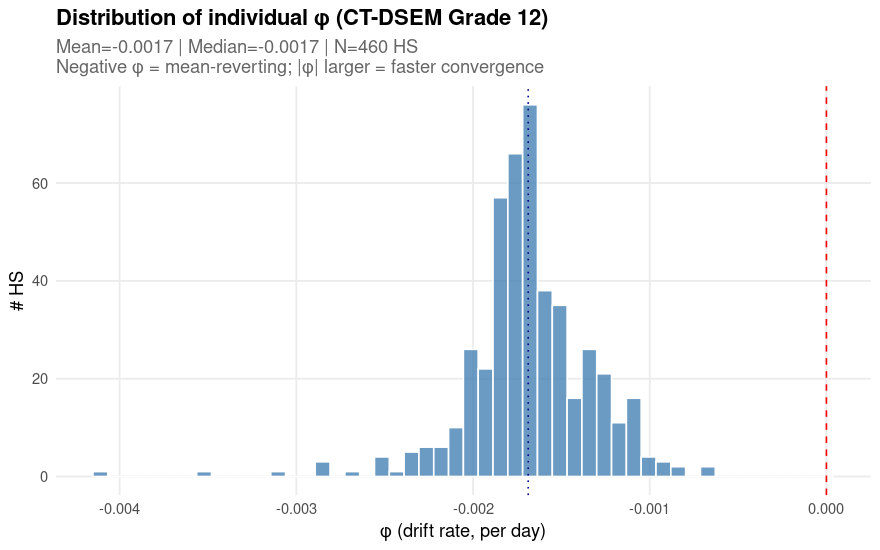
\includegraphics[width=1\linewidth]{../../outputs/b4_lsem/plots/ctdsem_phi_distribution} \caption{phi distribution}\label{fig:ctdsem-plots-1}
\end{figure}
\begin{figure}
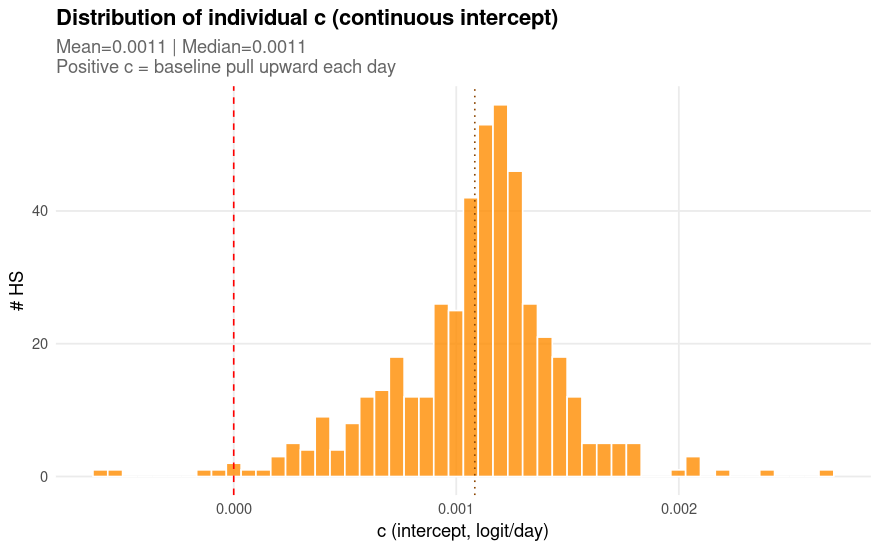
\includegraphics[width=1\linewidth]{../../outputs/b4_lsem/plots/ctdsem_cint_distribution} \caption{cint distribution}\label{fig:ctdsem-plots-2}
\end{figure}
\begin{figure}
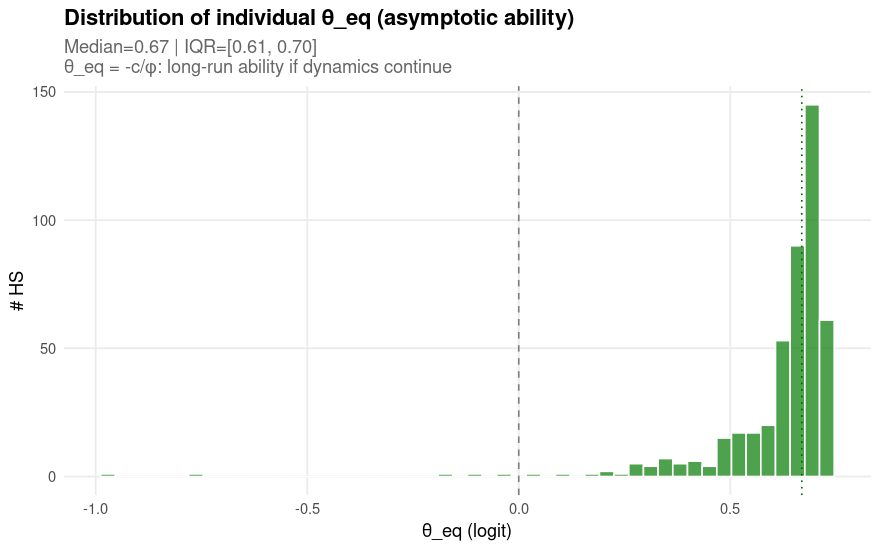
\includegraphics[width=1\linewidth]{../../outputs/b4_lsem/plots/ctdsem_theta_eq_distribution} \caption{theta_eq distribution}\label{fig:ctdsem-plots-3}
\end{figure}
\begin{figure}
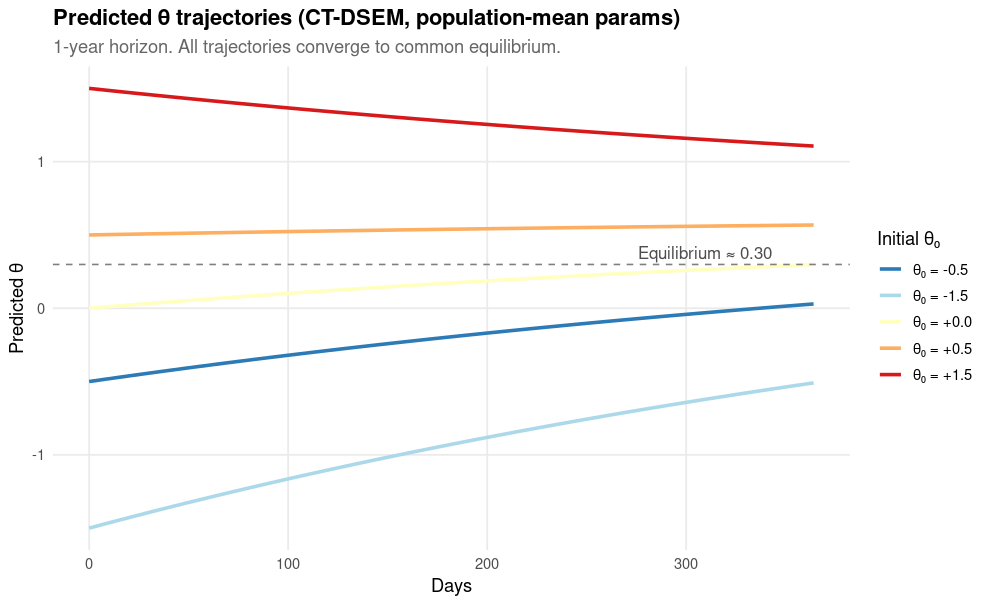
\includegraphics[width=1\linewidth]{../../outputs/b4_lsem/plots/ctdsem_predicted_trajectories} \caption{Predicted trajectories}\label{fig:ctdsem-plots-4}
\end{figure}
\begin{figure}
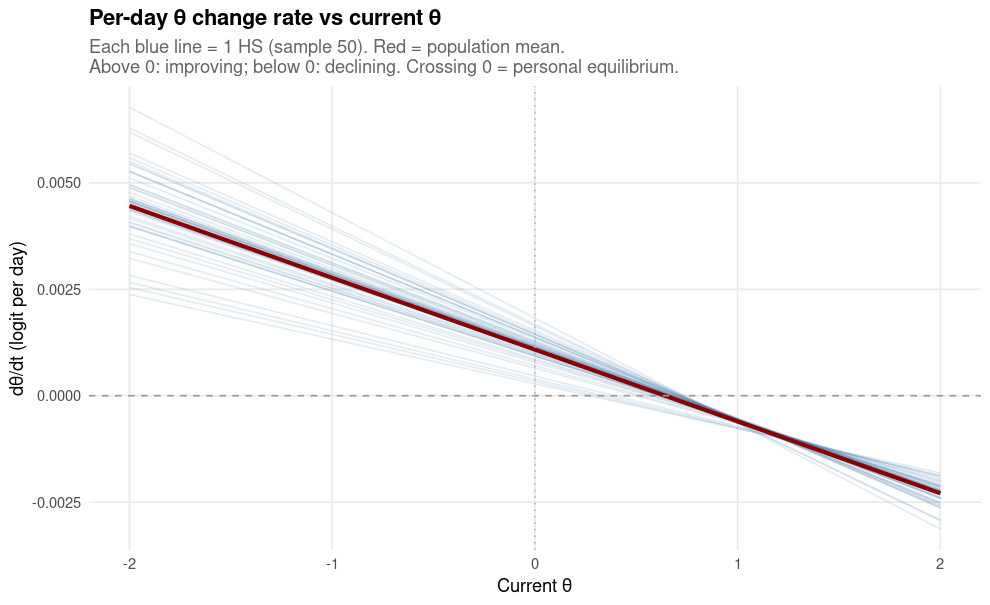
\includegraphics[width=1\linewidth]{../../outputs/b4_lsem/plots/ctdsem_rate_vs_theta} \caption{dtheta/dt vs current theta}\label{fig:ctdsem-plots-5}
\end{figure}

\hypertarget{kalman-smoothing-b6-real-time-online-layer}{%
\section{8. Kalman smoothing (B6) --- real-time / online
layer}\label{kalman-smoothing-b6-real-time-online-layer}}

The CT-DSEM model in §7 describes a continuous-time latent process;
\textbf{Kalman smoothing on the EAP series gives the discrete-time,
frequentist counterpart} --- a recursive estimator that can be deployed
in production for real-time ability tracking. Per occasion the state
evolves and the noisy EAP estimate \(\hat\theta_{it}\) updates the
filter:

\[
\theta_{it} = \theta_{i,t-1} + u_{it},\quad u_{it} \sim \mathcal{N}(0, q_g),\qquad
\hat\theta_{it} = \theta_{it} + \varepsilon_{it},\quad \varepsilon_{it} \sim \mathcal{N}(0, \mathrm{SE}_{it}^2).
\]

The observation variance is \emph{time-varying} --- it is the
per-occasion EAP standard error from B3, which is small when an HS
attempts many items on a day and large when they attempt few. The state
innovation variance \(q_g\) is pooled per grade by method of moments on
consecutive increments:
\(\widehat{q}_g = \overline{\Delta\hat\theta^2} - \overline{\mathrm{SE}_t^2 + \mathrm{SE}_{t-1}^2}\).

\begin{longtable}[]{@{}rrrrr@{}}
\caption{B6 Kalman gain --- mean SE before/after smoothing and pooled
state-innovation variance}\tabularnewline
\toprule
grade & mean\_se\_raw & mean\_se\_smooth & pct\_reduction &
q\_state\_variance \\
\midrule
\endfirsthead
\toprule
grade & mean\_se\_raw & mean\_se\_smooth & pct\_reduction &
q\_state\_variance \\
\midrule
\endhead
10 & 0.499 & 0.387 & 0.412 & 0.44417 \\
11 & 0.527 & 0.433 & 0.343 & 0.73396 \\
12 & 0.442 & 0.369 & 0.320 & 0.61959 \\
\bottomrule
\end{longtable}

\begin{figure}
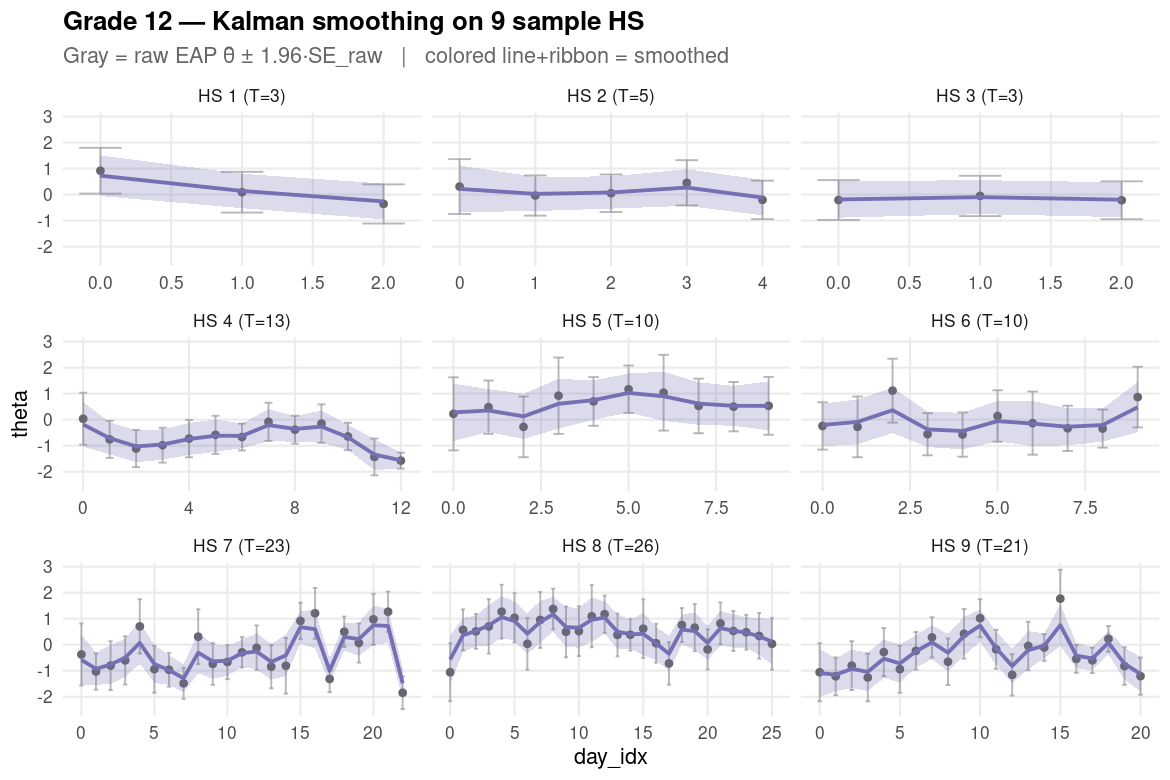
\includegraphics[width=0.49\linewidth]{../../outputs/b6_kalman/plots/kalman_overlay_grade_12} 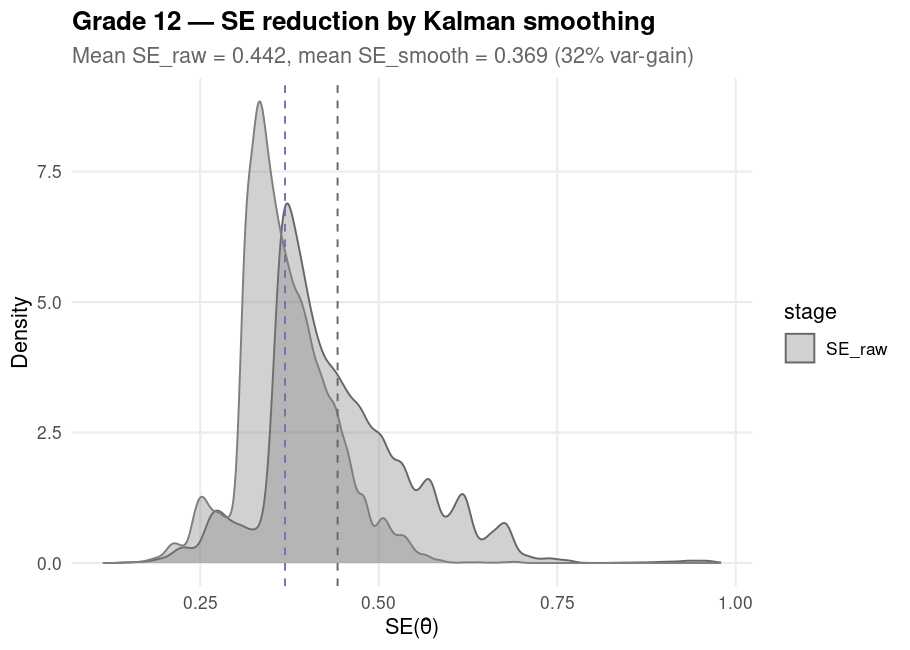
\includegraphics[width=0.49\linewidth]{../../outputs/b6_kalman/plots/kalman_se_reduction_grade_12} 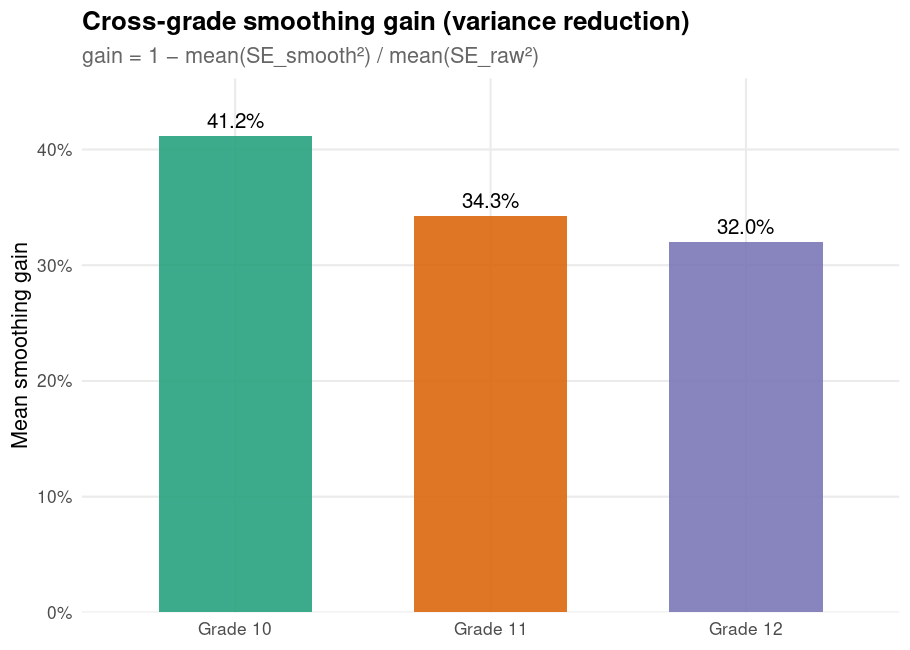
\includegraphics[width=0.49\linewidth]{../../outputs/b6_kalman/plots/kalman_pop_gain} \caption{Cross-grade variance smoothing gain.}\label{fig:kalman-plots}
\end{figure}

Kalman smoothing tightens per-occasion ability estimates most where they
are weakest: early occasions with few items per day. The variance
reduction (``smoothing gain'') quantifies how much measurement noise the
temporal model absorbs. This is the \textbf{online-estimation}
ingredient that addresses MT2 of the proposal; a streaming variational
generalisation that handles the logit observation directly (rather than
via the EAP intermediate) is documented as a design contribution in
\texttt{docs/oirt\_vi\_design.md} and listed as Phase 2 runtime work.
The smoothed trajectory is also re-used in §9 below as the lower-noise
input to the early-warning drop signal.

\hypertarget{applications-b7}{%
\section{9. Applications (B7)}\label{applications-b7}}

The two prototypes below convert the dynamic ability estimates into
concrete pedagogical signals --- a \emph{candidate list} for human
review (early warning) and a \emph{next-item} recommendation under the
1PL information-max policy. Neither is a deterministic classifier; both
are decision-support outputs intended to be embedded in the OLM platform
alongside teacher dashboards.

\hypertarget{early-warning-at-risk-hs-flagging}{%
\subsection{9.1 Early-warning --- at-risk HS
flagging}\label{early-warning-at-risk-hs-flagging}}

For each grade, an HS is flagged if \textbf{either} of two criteria
holds:

\begin{itemize}
\tightlist
\item
  \emph{Structural}: precision-weighted per-HS growth slope (from the
  B4a lmer fit, \texttt{fixef(day\_idx)\ +\ ranef\$iduser\$day\_idx}) is
  in the bottom 10\% of the cohort.
\item
  \emph{Event-level}: the largest single-step decrement on the
  \textbf{Kalman-smoothed} trajectory (§8),
  \(\min(\Delta\theta^{\text{smooth}}_{it})\), falls below \(-1.0\)
  logit. Computing the drop on the smoothed series rather than on the
  raw EAP \(\hat\theta_{it}\) matters: mean
  \(\mathrm{SE}_{\text{smooth}} \approx 0.40\) logit, so \(-1.0\)
  corresponds to \(\approx 2.5\,\mathrm{SE}\) --- a robust signal rather
  than a single-occasion bounce.
\end{itemize}

Eligible cohort: HS with \(T \geq 3\) measurements (so slope is
identifiable). The flag is intentionally unioned (OR) and accompanied by
a stricter AND variant in the per-grade CSVs --- the union casts a wide
net for follow-up, the intersection narrows to the most consistent
signals.

\begin{longtable}[]{@{}
  >{\raggedleft\arraybackslash}p{(\columnwidth - 12\tabcolsep) * \real{0.0882}}
  >{\raggedleft\arraybackslash}p{(\columnwidth - 12\tabcolsep) * \real{0.1176}}
  >{\raggedleft\arraybackslash}p{(\columnwidth - 12\tabcolsep) * \real{0.1471}}
  >{\raggedleft\arraybackslash}p{(\columnwidth - 12\tabcolsep) * \real{0.1765}}
  >{\raggedleft\arraybackslash}p{(\columnwidth - 12\tabcolsep) * \real{0.1912}}
  >{\raggedleft\arraybackslash}p{(\columnwidth - 12\tabcolsep) * \real{0.1765}}
  >{\raggedleft\arraybackslash}p{(\columnwidth - 12\tabcolsep) * \real{0.1029}}@{}}
\caption{Early-warning flag counts per grade (OR-flag = either slope or
drop; AND in n\_both)}\tabularnewline
\toprule
\begin{minipage}[b]{\linewidth}\raggedleft
grade
\end{minipage} & \begin{minipage}[b]{\linewidth}\raggedleft
n\_total
\end{minipage} & \begin{minipage}[b]{\linewidth}\raggedleft
n\_flagged
\end{minipage} & \begin{minipage}[b]{\linewidth}\raggedleft
pct\_flagged
\end{minipage} & \begin{minipage}[b]{\linewidth}\raggedleft
n\_slope\_only
\end{minipage} & \begin{minipage}[b]{\linewidth}\raggedleft
n\_drop\_only
\end{minipage} & \begin{minipage}[b]{\linewidth}\raggedleft
n\_both
\end{minipage} \\
\midrule
\endfirsthead
\toprule
\begin{minipage}[b]{\linewidth}\raggedleft
grade
\end{minipage} & \begin{minipage}[b]{\linewidth}\raggedleft
n\_total
\end{minipage} & \begin{minipage}[b]{\linewidth}\raggedleft
n\_flagged
\end{minipage} & \begin{minipage}[b]{\linewidth}\raggedleft
pct\_flagged
\end{minipage} & \begin{minipage}[b]{\linewidth}\raggedleft
n\_slope\_only
\end{minipage} & \begin{minipage}[b]{\linewidth}\raggedleft
n\_drop\_only
\end{minipage} & \begin{minipage}[b]{\linewidth}\raggedleft
n\_both
\end{minipage} \\
\midrule
\endhead
10 & 6285 & 905 & 14.40 & 411 & 276 & 218 \\
11 & 6740 & 1357 & 20.13 & 293 & 683 & 381 \\
12 & 10440 & 2325 & 22.27 & 557 & 1281 & 487 \\
\bottomrule
\end{longtable}

The flagged share rises from 14\% in Grade 10 to 22\% in Grade 12,
consistent with the catch-up→plateau story (more ``drops'' survive into
a regime where compensatory dynamics no longer absorb them). The
\texttt{n\_both} column gives the high-confidence subset that triggered
\emph{both} the slope and the drop criterion --- these are the most
defensible candidates for early intervention. Operationally these lists
would feed a queue for teacher review or for an automatic remediation
track on OLM; they are not endpoints in themselves.

\hypertarget{item-recommendation-1pl-information-max}{%
\subsection{9.2 Item recommendation --- 1PL
information-max}\label{item-recommendation-1pl-information-max}}

Under the 1PL Rasch model the Fisher information of item \(j\) at
ability \(\theta\) is

\[
I_j(\theta) \;=\; P_j(\theta)\bigl(1 - P_j(\theta)\bigr),\qquad P_j(\theta) = \sigma(\theta - b_j),
\]

maximised at \(b_j = \theta\) (peak value \(0.25\)). The recommender
returns the top-\(k\) items minimising
\(|b_j - \hat\theta_{\text{current}}|\) subject to
\(|b_j - \hat\theta| < \delta = 0.5\), which keeps information
\(\geq 0.235\) (≈94\% of peak).

For demonstration we pick 10 representative HS per grade --- 3 low
(\(\hat\theta \leq Q_{10}\)), 4 mid (\(Q_{40} < \hat\theta < Q_{60}\)),
3 high (\(\hat\theta \geq Q_{90}\)) --- with deterministic seed 42,
using each HS's most recent occasion in B3 as
\(\hat\theta_{\text{current}}\).

\begin{longtable}[]{@{}
  >{\raggedleft\arraybackslash}p{(\columnwidth - 16\tabcolsep) * \real{0.0594}}
  >{\raggedleft\arraybackslash}p{(\columnwidth - 16\tabcolsep) * \real{0.1485}}
  >{\raggedleft\arraybackslash}p{(\columnwidth - 16\tabcolsep) * \real{0.1386}}
  >{\raggedright\arraybackslash}p{(\columnwidth - 16\tabcolsep) * \real{0.0792}}
  >{\raggedleft\arraybackslash}p{(\columnwidth - 16\tabcolsep) * \real{0.0891}}
  >{\raggedright\arraybackslash}p{(\columnwidth - 16\tabcolsep) * \real{0.1485}}
  >{\raggedleft\arraybackslash}p{(\columnwidth - 16\tabcolsep) * \real{0.0990}}
  >{\raggedleft\arraybackslash}p{(\columnwidth - 16\tabcolsep) * \real{0.0990}}
  >{\raggedleft\arraybackslash}p{(\columnwidth - 16\tabcolsep) * \real{0.1386}}@{}}
\caption{Top-3 recommendations for the first 5 demo HS --- preview (full
table in final\_recommendation\_examples.csv).}\tabularnewline
\toprule
\begin{minipage}[b]{\linewidth}\raggedleft
grade
\end{minipage} & \begin{minipage}[b]{\linewidth}\raggedleft
iduser
\end{minipage} & \begin{minipage}[b]{\linewidth}\raggedleft
theta\_current
\end{minipage} & \begin{minipage}[b]{\linewidth}\raggedright
profile
\end{minipage} & \begin{minipage}[b]{\linewidth}\raggedleft
rec\_rank
\end{minipage} & \begin{minipage}[b]{\linewidth}\raggedright
question\_id
\end{minipage} & \begin{minipage}[b]{\linewidth}\raggedleft
b
\end{minipage} & \begin{minipage}[b]{\linewidth}\raggedleft
abs\_diff
\end{minipage} & \begin{minipage}[b]{\linewidth}\raggedleft
info\_at\_theta
\end{minipage} \\
\midrule
\endfirsthead
\toprule
\begin{minipage}[b]{\linewidth}\raggedleft
grade
\end{minipage} & \begin{minipage}[b]{\linewidth}\raggedleft
iduser
\end{minipage} & \begin{minipage}[b]{\linewidth}\raggedleft
theta\_current
\end{minipage} & \begin{minipage}[b]{\linewidth}\raggedright
profile
\end{minipage} & \begin{minipage}[b]{\linewidth}\raggedleft
rec\_rank
\end{minipage} & \begin{minipage}[b]{\linewidth}\raggedright
question\_id
\end{minipage} & \begin{minipage}[b]{\linewidth}\raggedleft
b
\end{minipage} & \begin{minipage}[b]{\linewidth}\raggedleft
abs\_diff
\end{minipage} & \begin{minipage}[b]{\linewidth}\raggedleft
info\_at\_theta
\end{minipage} \\
\midrule
\endhead
10 & 16386157283336 & 1.774258 & high & 1 & 202447173702 & 1.779805 &
0.0055469 & 0.2499981 \\
10 & 16386157283336 & 1.774258 & high & 2 & 205204801303 & 1.767689 &
0.0065687 & 0.2499973 \\
10 & 16386157283336 & 1.774258 & high & 3 & 205541087413\_d & 1.759586 &
0.0146723 & 0.2499865 \\
10 & 16391550896809 & 1.301467 & high & 1 & 200320925171 & 1.293413 &
0.0080542 & 0.2499959 \\
10 & 16391550896809 & 1.301467 & high & 2 & 202497722231\_a & 1.317738 &
0.0162709 & 0.2499835 \\
10 & 16391550896809 & 1.301467 & high & 3 & 204472041935\_l & 1.325199 &
0.0237314 & 0.2499648 \\
10 & 16401844077601 & 1.693749 & high & 1 & 205340803431 & 1.698383 &
0.0046340 & 0.2499987 \\
10 & 16401844077601 & 1.693749 & high & 2 & 203745260100 & 1.673855 &
0.0198933 & 0.2499753 \\
10 & 16401844077601 & 1.693749 & high & 3 & 203601876707 & 1.668229 &
0.0255198 & 0.2499593 \\
10 & 16385598633612 & -1.886709 & low & 1 & 200541050487 & -1.886576 &
0.0001333 & 0.2500000 \\
10 & 16385598633612 & -1.886709 & low & 2 & 204273005335 & -1.886527 &
0.0001824 & 0.2500000 \\
10 & 16385598633612 & -1.886709 & low & 3 & 200787681114 & -1.887820 &
0.0011113 & 0.2499999 \\
10 & 16399578653481 & -1.957081 & low & 1 & 200211075479 & -1.957853 &
0.0007718 & 0.2500000 \\
10 & 16399578653481 & -1.957081 & low & 2 & 205111529802\_c & -1.956179
& 0.0009023 & 0.2499999 \\
10 & 16399578653481 & -1.957081 & low & 3 & 202429718876 & -1.955959 &
0.0011222 & 0.2499999 \\
\bottomrule
\end{longtable}

\textbf{Caveats.} (a) \emph{Cold start}: a brand-new HS has no
\(\hat\theta\), so the recommender must default to the EAP prior
(\(\theta=0\)) until at least one response arrives. (b) \emph{No
content-area diversity}: this prototype optimises only on measurement
information, not on syllabus coverage; a production version would
combine information-max with a coverage constraint over the OLM topic
taxonomy. (c) \emph{Static item bank}: the recommendation uses the
2024-25 calibrated \(b_j\) values; Phase 2 will add online recalibration
as new responses accumulate.

\hypertarget{cross-grade-pattern}{%
\section{10. Cross-grade Pattern}\label{cross-grade-pattern}}

\begin{verbatim}
## LGCM slopes across grades: g10=0.0146, g11=0.0281, g12=0.0058
\end{verbatim}

\begin{verbatim}
## Coefficient of variation (CV) = 0.69
\end{verbatim}

\begin{verbatim}
## Pre-registered threshold: CV < 0.30. Result: FAIL
\end{verbatim}

\begin{verbatim}
## All slopes positive: YES
\end{verbatim}

\textbf{Cross-grade pattern assessment} (reframing pre-registered
thresholds as findings, not failures):

\begin{itemize}
\tightlist
\item
  \textbf{Direction}: all 3 grades show positive growth --- the most
  robust, fully consistent result.
\item
  \textbf{Magnitude / CV}: the CV \textless{} 0.30 threshold is not met.
  With slopes in the 0.006--0.028 range, small absolute differences
  inflate relative variation; the cross-grade differences (Grade 11
  active growth vs Grade 12 ceiling effects) are \textbf{substantively
  interpretable}, not measurement instability.
\item
  \textbf{Coupling}: the catch-up → plateau shift (\(\beta\) negative in
  Grade 10, \(\approx 0\) in Grade 12) is itself the key cross-grade
  \emph{finding} --- a qualitative regime change, consistent with
  content becoming more cumulative in upper grades.
\end{itemize}

The threshold ``failures'' are therefore reported as substantive
results, following the reframing in the table below (§12), rather than
as problems with the measurement model.

\hypertarget{discussion}{%
\section{11. Discussion}\label{discussion}}

\hypertarget{the-compensatory-to-plateau-shift}{%
\subsection{11.1 The compensatory-to-plateau
shift}\label{the-compensatory-to-plateau-shift}}

The most striking result is a \emph{qualitative shift} in ability
dynamics across grades. In Grade 10 the LCSM coupling is clearly
negative (\(\beta = -0.069\)), so students with lower initial ability
gain disproportionately more --- a \textbf{compensatory (catch-up)}
regime that narrows the within-grade gap. By Grade 11 this effect is
marginal (\(\beta = -0.043\), CI crosses 0), and by Grade 12 it vanishes
(\(\beta \approx 0\)): students preserve their relative positions --- a
\textbf{plateau} regime. The continuous-time Grade 12 model tells the
same story from a different angle: a mean-reverting process with
equilibrium \(\theta_{\text{eq}} = -c/\varphi \approx 0.65\) logit and a
long half-life (\(\approx 408\) days), i.e.~weak pull toward a common
level.

\hypertarget{pedagogical-implications}{%
\subsection{11.2 Pedagogical
implications}\label{pedagogical-implications}}

The grade-differential pattern suggests \textbf{intervention timing
matters}. Remedial support is likely most effective in Grade 10, where
compensatory dynamics already operate in students' favour; by Grade 12
the system shifts toward preserving existing gaps, so the same gain
requires more intensive, earlier intervention. The continuous-time
estimate that low-ability students gain \(\approx 0.25\) logit per
semester (vs slight regression for high-ability students) gives a
concrete, time-scaled target for monitoring.

\hypertarget{methodological-contributions-multi-tier-convergent-design}{%
\subsection{11.3 Methodological contributions (multi-tier convergent
design)}\label{methodological-contributions-multi-tier-convergent-design}}

This study contributes a \textbf{multi-tier convergent design} for
dynamic ability: (Tier 1) LGCM/LCSM with bootstrap CIs on a capped,
balanced window; (Tier 2) precision-weighted and unweighted
mixed-effects models on the full, unbalanced data; (Tier 3) a
continuous-time DSEM for the intensively-measured subsample; and (Tier
4) a Kalman state-space smoother that turns the same EAP series into a
real-time, frequentist counterpart of Tier 3 (B6, §8). Agreement on the
\emph{direction} of growth across all tiers --- despite different data
coverage and estimators --- is stronger evidence than any single model,
and the residual LGCM--lmer slope gap is transparently attributed to
FIML-vs-REML method effects rather than to substantive nonlinearity. The
Kalman layer also feeds two downstream applications (§9), closing the
loop from measurement to actionable signal.

\hypertarget{comparison-with-literature}{%
\subsection{11.4 Comparison with
literature}\label{comparison-with-literature}}

The catch-up coupling sign in lower grades is consistent with
compensatory growth reported in the LCSM literature (McArdle, 2009),
while the move toward a Matthew/plateau regime in cumulative upper-grade
content echoes findings on widening gaps when prerequisites compound.
The continuous-time framing follows Driver, Oud \& Voelkle (2017) and
Asparouhov, Hamaker \& Muthén (2018); using IRT EAP scores with their
measurement error as input to the structural layer is the bridge that
makes per-occasion ability usable in these models.

\hypertarget{limitations-caveats}{%
\section{12. Limitations \& Caveats}\label{limitations-caveats}}

\begin{enumerate}
\def\labelenumi{\arabic{enumi}.}
\item
  \textbf{Itemfit S-X2 unavailable} for any grade due to sparse response
  patterns (each HS attempts ≪ 10\% of the item pool). X2/infit was
  substituted as the misfit screen.
\item
  \textbf{B4a bootstrap nonadmissibility} was high for LGCM grade 10
  (68.6\%) and grade 12 (84.9\%). LGCM CIs for these grades should be
  interpreted as suggestive; lmer Tier 2 provides primary inference.
\item
  \textbf{LGCM-lmer convergent evidence} failed the pre-registered
  \(|\Delta| < 0.005\) threshold for all grades. Sensitivity analysis
  attributes this to method (FIML linear-growth imputation vs REML on
  observed cases) rather than nonlinear growth --- interpreted as a
  substantive method effect, not a measurement problem.
\item
  \textbf{CT-DSEM uses MAP estimation} (\texttt{optim} mode) for point
  estimates with Wald-type CIs. Full Bayesian MCMC remains as future
  sensitivity check.
\item
  \textbf{2PL EAP scoring not done} as primary; 1PL Rasch was used due
  to 2-6\% degenerate items (\(a \le 0\) or \(|b| > 5\)) in 2PL fits.
  2PL kept for future sensitivity.
\item
  \textbf{Phase 1 only}: This report covers school year 2024-2025.
  Cross-year linking and trends are out of scope.
\item
  \textbf{Per-grade calibration}: No cross-grade theta scale linking.
  Inferences within grades only --- cross-grade comparisons are
  qualitative (pattern shifts), not quantitative magnitude comparisons.
\item
  \textbf{No teacher/class metadata}: the OLM math collections
  (\texttt{math\_teacher\_static}, \texttt{math\_teacher\_categories},
  \texttt{math\_teacher\_course}) do not contain a \texttt{class\_id} /
  \texttt{teacher\_id} / \texttt{school\_id} field, so the proposal's
  MT4(c) \emph{teaching-effectiveness} analysis is deferred to Phase 2
  pending schema enrichment. See \texttt{docs/scope\_refinement.md}.
\item
  \textbf{Single-construct measurement → no RI-CLPM}: the proposal lists
  RI-CLPM among four LSEM variants, but RI-CLPM requires ≥2 constructs
  measured longitudinally to identify cross-lagged effects; Phase 1 has
  only mathematics ability, so RI-CLPM is over-specified and was dropped
  on methodological grounds rather than for lack of time.
\item
  \textbf{VI/OIRT delivered as a design contribution only}: the
  streaming variational form of MT2 needs a deployment platform (the
  proposal's §8.3 production code is also deferred). The algorithmic
  specification --- ELBO, streaming update, complexity --- is documented
  in \texttt{docs/oirt\_vi\_design.md}.
\end{enumerate}

\hypertarget{conclusion}{%
\section{13. Conclusion}\label{conclusion}}

Integrating IRT with longitudinal SEM enables tracking of \emph{dynamic}
math ability on a Vietnamese online learning system. Across grades
10--12 we find consistent, small, positive growth (RQ1) and a robust
\textbf{catch-up → plateau shift} (RQ3): a compensatory regime in Grade
10 that weakens through Grade 11 and disappears by Grade 12,
corroborated by a continuous-time mean-reversion model. The dynamics are
directionally consistent across grades and estimation methods (RQ2),
while the differences in magnitude are substantively interpretable
rather than artefacts. These results carry a direct pedagogical message
--- intervene early, while compensatory dynamics still help --- and lay
the methodological groundwork for Phase 2 (cross-year vertical scaling
with the 2025-2026 review course as natural anchor items).

Two downstream applications translate the dynamic estimates into
actionable signals for the OLM platform: a real-time Kalman smoothing
layer (B6) that tightens per-occasion ability estimates by absorbing
measurement noise across time, and prototype early-warning +
item-recommendation tools (B7) that surface at-risk students and serve
information-maximising next items.

\hypertarget{reproducibility}{%
\section{14. Reproducibility}\label{reproducibility}}

Pipeline scripts in \texttt{research/irt\_lsem/src/r/}:

\begin{longtable}[]{@{}lll@{}}
\toprule
Script & Step & Runtime \\
\midrule
\endhead
\texttt{b1\_dimensionality.R} & B1 & \textasciitilde30 min \\
\texttt{b2\_calibration.R} & B2 & \textasciitilde3 hours \\
\texttt{b2\_postprocess.R} & B2 cleanup & \textasciitilde5 min \\
\texttt{b3\_eap\_scoring.R} & B3 & \textasciitilde20 min \\
\texttt{b4a\_lgcm\_lcsm.R} & B4a & \textasciitilde17 min \\
\texttt{b4a\_test.R} & B4a sensitivity & \textasciitilde2 min \\
\texttt{b4c\_ctdsem.R} & B4c & \textasciitilde2 min (optim) \\
\texttt{b4c\_viz.R} & B4c plots & \textasciitilde1 min \\
\texttt{b5\_consolidate.R} & B5 tables & \textless1 min \\
\texttt{b5\_plots.R} & B5 figures & \textless1 min \\
\texttt{b6\_kalman.R} & B6 KFAS smoother & \textasciitilde2 min \\
\texttt{b6\_viz.R} & B6 plots & \textless1 min \\
\texttt{b7a\_early\_warning.R} & B7a flagging & \textless1 min \\
\texttt{b7b\_recommendation.R} & B7b recommender & \textless1 min \\
\texttt{b5\_report.Rmd} & this document & \textless1 min \\
\bottomrule
\end{longtable}

Outputs are CSV/RDS/PNG; all artefacts in \texttt{outputs/}. R version R
version 4.5.2 (2025-10-31). Random seed = 42 across pipeline.

\begin{verbatim}
## R version 4.5.2 (2025-10-31)
## Platform: x86_64-pc-linux-gnu
## Running under: Debian GNU/Linux 12 (bookworm)
## 
## Matrix products: default
## BLAS:   /usr/lib/x86_64-linux-gnu/openblas-pthread/libblas.so.3 
## LAPACK: /usr/lib/x86_64-linux-gnu/openblas-pthread/libopenblasp-r0.3.21.so;  LAPACK version 3.11.0
## 
## locale:
##  [1] LC_CTYPE=en_US.UTF-8       LC_NUMERIC=C              
##  [3] LC_TIME=en_US.UTF-8        LC_COLLATE=en_US.UTF-8    
##  [5] LC_MONETARY=en_US.UTF-8    LC_MESSAGES=en_US.UTF-8   
##  [7] LC_PAPER=en_US.UTF-8       LC_NAME=C                 
##  [9] LC_ADDRESS=C               LC_TELEPHONE=C            
## [11] LC_MEASUREMENT=en_US.UTF-8 LC_IDENTIFICATION=C       
## 
## time zone: Asia/Bangkok
## tzcode source: system (glibc)
## 
## attached base packages:
## [1] stats     graphics  grDevices utils     datasets  methods   base     
## 
## other attached packages:
## [1] knitr_1.50        data.table_1.17.6
## 
## loaded via a namespace (and not attached):
##  [1] bit_4.6.0         compiler_4.5.2    fastmap_1.2.0     cli_3.6.5        
##  [5] tools_4.5.2       htmltools_0.5.8.1 yaml_2.3.10       bit64_4.6.0-1    
##  [9] rmarkdown_2.29    xfun_0.52         digest_0.6.37     rlang_1.1.6      
## [13] evaluate_1.0.4
\end{verbatim}

\end{document}
